\documentclass[dvipdfmx,lettersize,journal]{IEEEtran}

\usepackage[ruled, vlined]{algorithm2e}    % \begin{algorithm2e}
\usepackage{amsmath}        % \begin{align*}
\usepackage{amssymb}        % \mathbb{A}
\usepackage{amsthm}         % \newtheorem
\usepackage{bm,bbm}         % \bm{A}, \bbm{1}
\usepackage{booktabs}       % \toprule, \midrule, \bottomrule
\usepackage{caption}        % \captionsetup
\usepackage{enumitem}       % \begin{enumerate}[label=(\alph*)]
\usepackage[dvipdfmx]{hyperref}       % \href{URL}{text}
\usepackage{ifthen}         % \ifthenelse
\usepackage{lipsum}         % \lipsum
\usepackage{mathrsfs}       % \mathscr{A}
\usepackage{mathtools}      % \mathrlap
\usepackage{optidef}        % \begin{mini*}{x}{f(x)}{}{}
\usepackage{orcidlink}      % \orcidlink
\usepackage{physics}        % \qty, \norm, \abs
\usepackage{subfiles}       % \subfile{file}
\usepackage{thm-restate}    % \begin{restatable}{theorem}{thm}
\usepackage{tikz}           % \begin{tikzpicture}
\usepackage{xparse}         % \NewDocumentCommand
% \usepackage{calc}         % \setlength
% \usepackage{cancel}       % \cancel
% \usepackage{parskip}      % \setlength{\parskip}{0.5em}
% \usepackage{csvsimple}    % \csvautotabular
% \usepackage{diagbox}      % \diagbox
% \usepackage{dsfont}       % \mathds{1}
% \usepackage{epsfig}       % \epsfig
% \usepackage{fancybx}      % \ovalbox
% \usepackage{float}        % \begin{figure}[H]
% \usepackage{lipsum}       % \lipsum
% \usepackage{listings}     % \begin{lstlisting}
\usepackage{makecell}     % \makecell{L1\L2}
% \usepackage{multicol}     % \begin{multicols}{2}
% \usepackage{multirow}     % \multirow
% \usepackage{nicematrix}   % \begin{NiceMatrix}
% \usepackage{qcircuit}     % \Qcircuit
% \usepackage{siunitx}      % \SI{1}{\second}
% \usepackage{stfloats}     % \begin{figure*}
% \usepackage{subcaption}   % \begin{subfigure}
% \usepackage{ulem}         % \sout
% \usepackage{wrapfig}      % \begin{wrapfigure}
% \usepackage[all]{xy}      % \xymatrix
% \usepackage[dvipdfmx]{graphicx}
% \usepackage[square, sort, comma, numbers]{natbib}

\hypersetup{colorlinks=true,linkcolor=blue,citecolor=blue,urlcolor=blue}

\definecolor{cA}{HTML}{0072BD}
\definecolor{cB}{HTML}{EDB120}
\definecolor{cC}{HTML}{77AC30}
\definecolor{cD}{HTML}{D95319}

\newcommand{\red}[1]{\textcolor{red}{#1}}
\newcommand{\blue}[1]{\textcolor{blue}{#1}}
\newcommand{\cyan}[1]{\textcolor{cyan}{#1}}
\newcommand{\gray}[1]{\textcolor{gray}{#1}}
\newcommand{\green}[1]{\textcolor{green}{#1}}
\newcommand{\brown}[1]{\textcolor{brown}{#1}}
\newcommand{\black}[1]{\textcolor{black}{#1}}
\newcommand{\orange}[1]{\textcolor{orange}{#1}}
\newcommand{\st}{\text{ s.t. }}
\newcommand{\Img}[1]{\mathrm{Im}\qty(#1)}
\newcommand{\Ker}[1]{\mathrm{Ker}\qty(#1)}
\newcommand{\Supp}[1]{\mathrm{supp}\qty(#1)}
\newcommand{\Rank}[1]{\mathrm{rank}\qty(#1)}
\newcommand{\floor}[1]{\left\lfloor #1 \right\rfloor}
\newcommand{\ceil}[1]{\left\lceil #1 \right\rceil}
% C++ (https://tex.stackexchange.com/questions/4302/prettiest-way-to-typeset-c-cplusplus)
\newcommand{\Cpp}{C\nolinebreak[4]\hspace{-.05em}\raisebox{.4ex}{\relsize{-3}{\textbf{++}}}}
% https://tex.stackexchange.com/questions/28836/typesetting-the-define-equals-symbol
\newcommand{\defeq}{\coloneqq}
\newcommand{\eqdef}{\eqqcolon}
% https://tex.stackexchange.com/questions/5502/how-to-get-a-mid-binary-relation-that-grows
\newcommand{\relmiddle}[1]{\mathrel{}\middle#1\mathrel{}}

% https://tex.stackexchange.com/questions/564216/newcommand-for-each-letter
\ExplSyntaxOn
\NewDocumentCommand{\definealphabet}{mmmm}{
\int_step_inline:nnn{`#3}{`#4}{
\cs_new_protected:cpx{#1 \char_generate:nn{##1}{11}}{
\exp_not:N #2{\char_generate:nn{##1}{11}}}}}
\ExplSyntaxOff

\definealphabet{bb}{\mathbb}{A}{Z}
\definealphabet{rm}{\mathrm}{A}{Z}
\definealphabet{cal}{\mathcal}{A}{Z}
\definealphabet{frak}{\mathfrak}{a}{z}
% \definealphabet{scr}{\mathscr}{A}{Z}
% \definealphabet{frak}{\mathfrak}{A}{Z}

\newtheorem{theorem}{Theorem}
\newtheorem{proposition}{Proposition}
\newtheorem{lemma}{Lemma}
\newtheorem{definition}{Definition}
\newtheorem{corollary}{Corollary}
\newtheorem{remark}{Remark}
\newtheorem{example}{Example}
\newtheorem{assumption}{Assumption}

% https://qiita.com/rityo_masu/items/efd44bc8f9229e014237
\allowdisplaybreaks[4]

\usetikzlibrary{
  3d,
  % fit,
  calc,
  math,
  matrix,
  patterns,
  backgrounds,
  arrows.meta,
  shapes.geometric,
  decorations.pathmorphing,
}


% \providecommand{\main}{.}
\newboolean{isMain}
\setboolean{isMain}{true}

\begin{document}
\bstctlcite{IEEEexample:BSTcontrol}

\title{Fruchterman--Reingold Layout with\\Subspace Method as Initial Placement}
\author{
  \orcidlinki{Hiroki Hamaguchi}{0009-0005-7348-1356} % TODO: fix
  \orcidlinki{Naoki Marumo}{0000-0002-7372-4275} % ? maybe dvipdfmx problem
  Akiko Takeda
  % <-this % stops a space
}
\maketitle

\begin{abstract}
  日本語で書かれている場合、執筆中を表す。
  \orange{オレンジの文章は正確性が疑問視される記述やTODOな記述。}
  \blue{また、orcidlinkが壊れているのでauthorのところで暫定措置を取っているが、これは日本語を全削除してdvipdfmxを取り除けばok。}
  \lipsum[1]
\end{abstract}

\begin{IEEEkeywords}
  Graph Drawing, Optimization, Fruchterman--Reingold Layout, Random Subspace Method.
\end{IEEEkeywords}

\section{Introduction}\label{sec:introduction}

\IEEEPARstart{G}{raph} is a mathematical structure representing pairwise relationships between objects, and graph drawing is one of the most fundamental tasks in data science. Indeed, numerous kinds of algorithms have been proposed for graph drawing~\cite{tutteHowDrawGraph1963,chrobakLineartimeAlgorithmDrawing1995,sugiyamaMethodsVisualUnderstanding1981,ghassemitoosiSimulatedAnnealingPreProcessing2016}.
Among these, one of the most popular strategies is force-directed algorithms.

In force-directed algorithms, we model a graph as a system of particles with forces acting between them.
This class of algorithms includes the Kamada--Kawai (KK) layout~\cite{kamadaAlgorithmDrawingGeneral1989},
Eades' spring embedder~\cite{eades1984heuristic}, and the Fruchterman--Reingold (FR) layout~\cite{fruchtermanGraphDrawingForcedirected1991,kobourovSpringEmbeddersForce2012}, which serves as the central focus of this study.

The FR algorithm is one of the most widely used force-directed algorithms. It is also implemented in many modern graph drawing libraries such as NetworkX~\cite{osti_960616}, Graphviz~\cite{ellsonGraphvizOpenSource2002}, and igraph~\cite{csardiIgraphSoftwarePackage2006}.

However, both the KK layout and the FR layout suffer from high computational complexity, specifically $\order{\abs{V}^2}$ per iteration as it is, where $\abs{V}$ denotes the number of vertices. This computational burden makes it difficult to apply these algorithms to large-scale graphs.

To address this kind of burden, several methods have been developed. These include approximating the $n$-body simulation using multipole expansions~\cite{greengardFastAlgorithmParticle1987} or the Barnes--Hut approximation~\cite{barnesHierarchicalLogForcecalculation1986}, gradually refining the layouts using a multilevel approach~\cite{Hu2006EfficientHF} and employing stress majorization~\cite{gansnerGraphDrawingStress2005}.

Another approach is to directly accelerate the optimization process, which aligns with the aim of our work. Recent researches have accelerated the algorithms for FR layout or KK layout through various methods, including adaptation to GPU parallel architectures~\cite{gajdosParallelFruchtermanReingold2016}, utilizing numerical optimization techniques such as L-BFGS~\cite{6183577}, and Stochastic Gradient Descent (SGD)~\cite{8419285}.

Based on such advances, in this paper, we investigate the ability of another algorithm: subspace methods.
Subspace methods are a class of optimization algorithms that restrict the optimization to a lower-dimensional subspace of the solution space, which can significantly reduce the computational cost per iteration.
We propose a new algorithm for the FR layout that leverages the subspace method, and we demonstrate its effectiveness through experiments.

The rest of the paper is organized as follows.
In Section~\ref{sec:preliminary}, we define the optimization problem for the FR algorithm.
In Section~\ref{sec:RQ}, we present our research question based on previous works.
In Section~\ref{sec:algorithm}, we propose a new algorithm that utilizes the subspace method for the FR layout.
In Section~\ref{sec:experiment}, we present our experimental results.
Finally, we conclude and discuss future work in Section~\ref{sec:discussion}.

\begin{figure}[t]
  \centering
  \begin{tabular}{cc}
    \large{\textbf{FR}}                           & \large{\textbf{L-BFGS}}   \\
    \begin{minipage}{0.45\columnwidth}
      \centering
      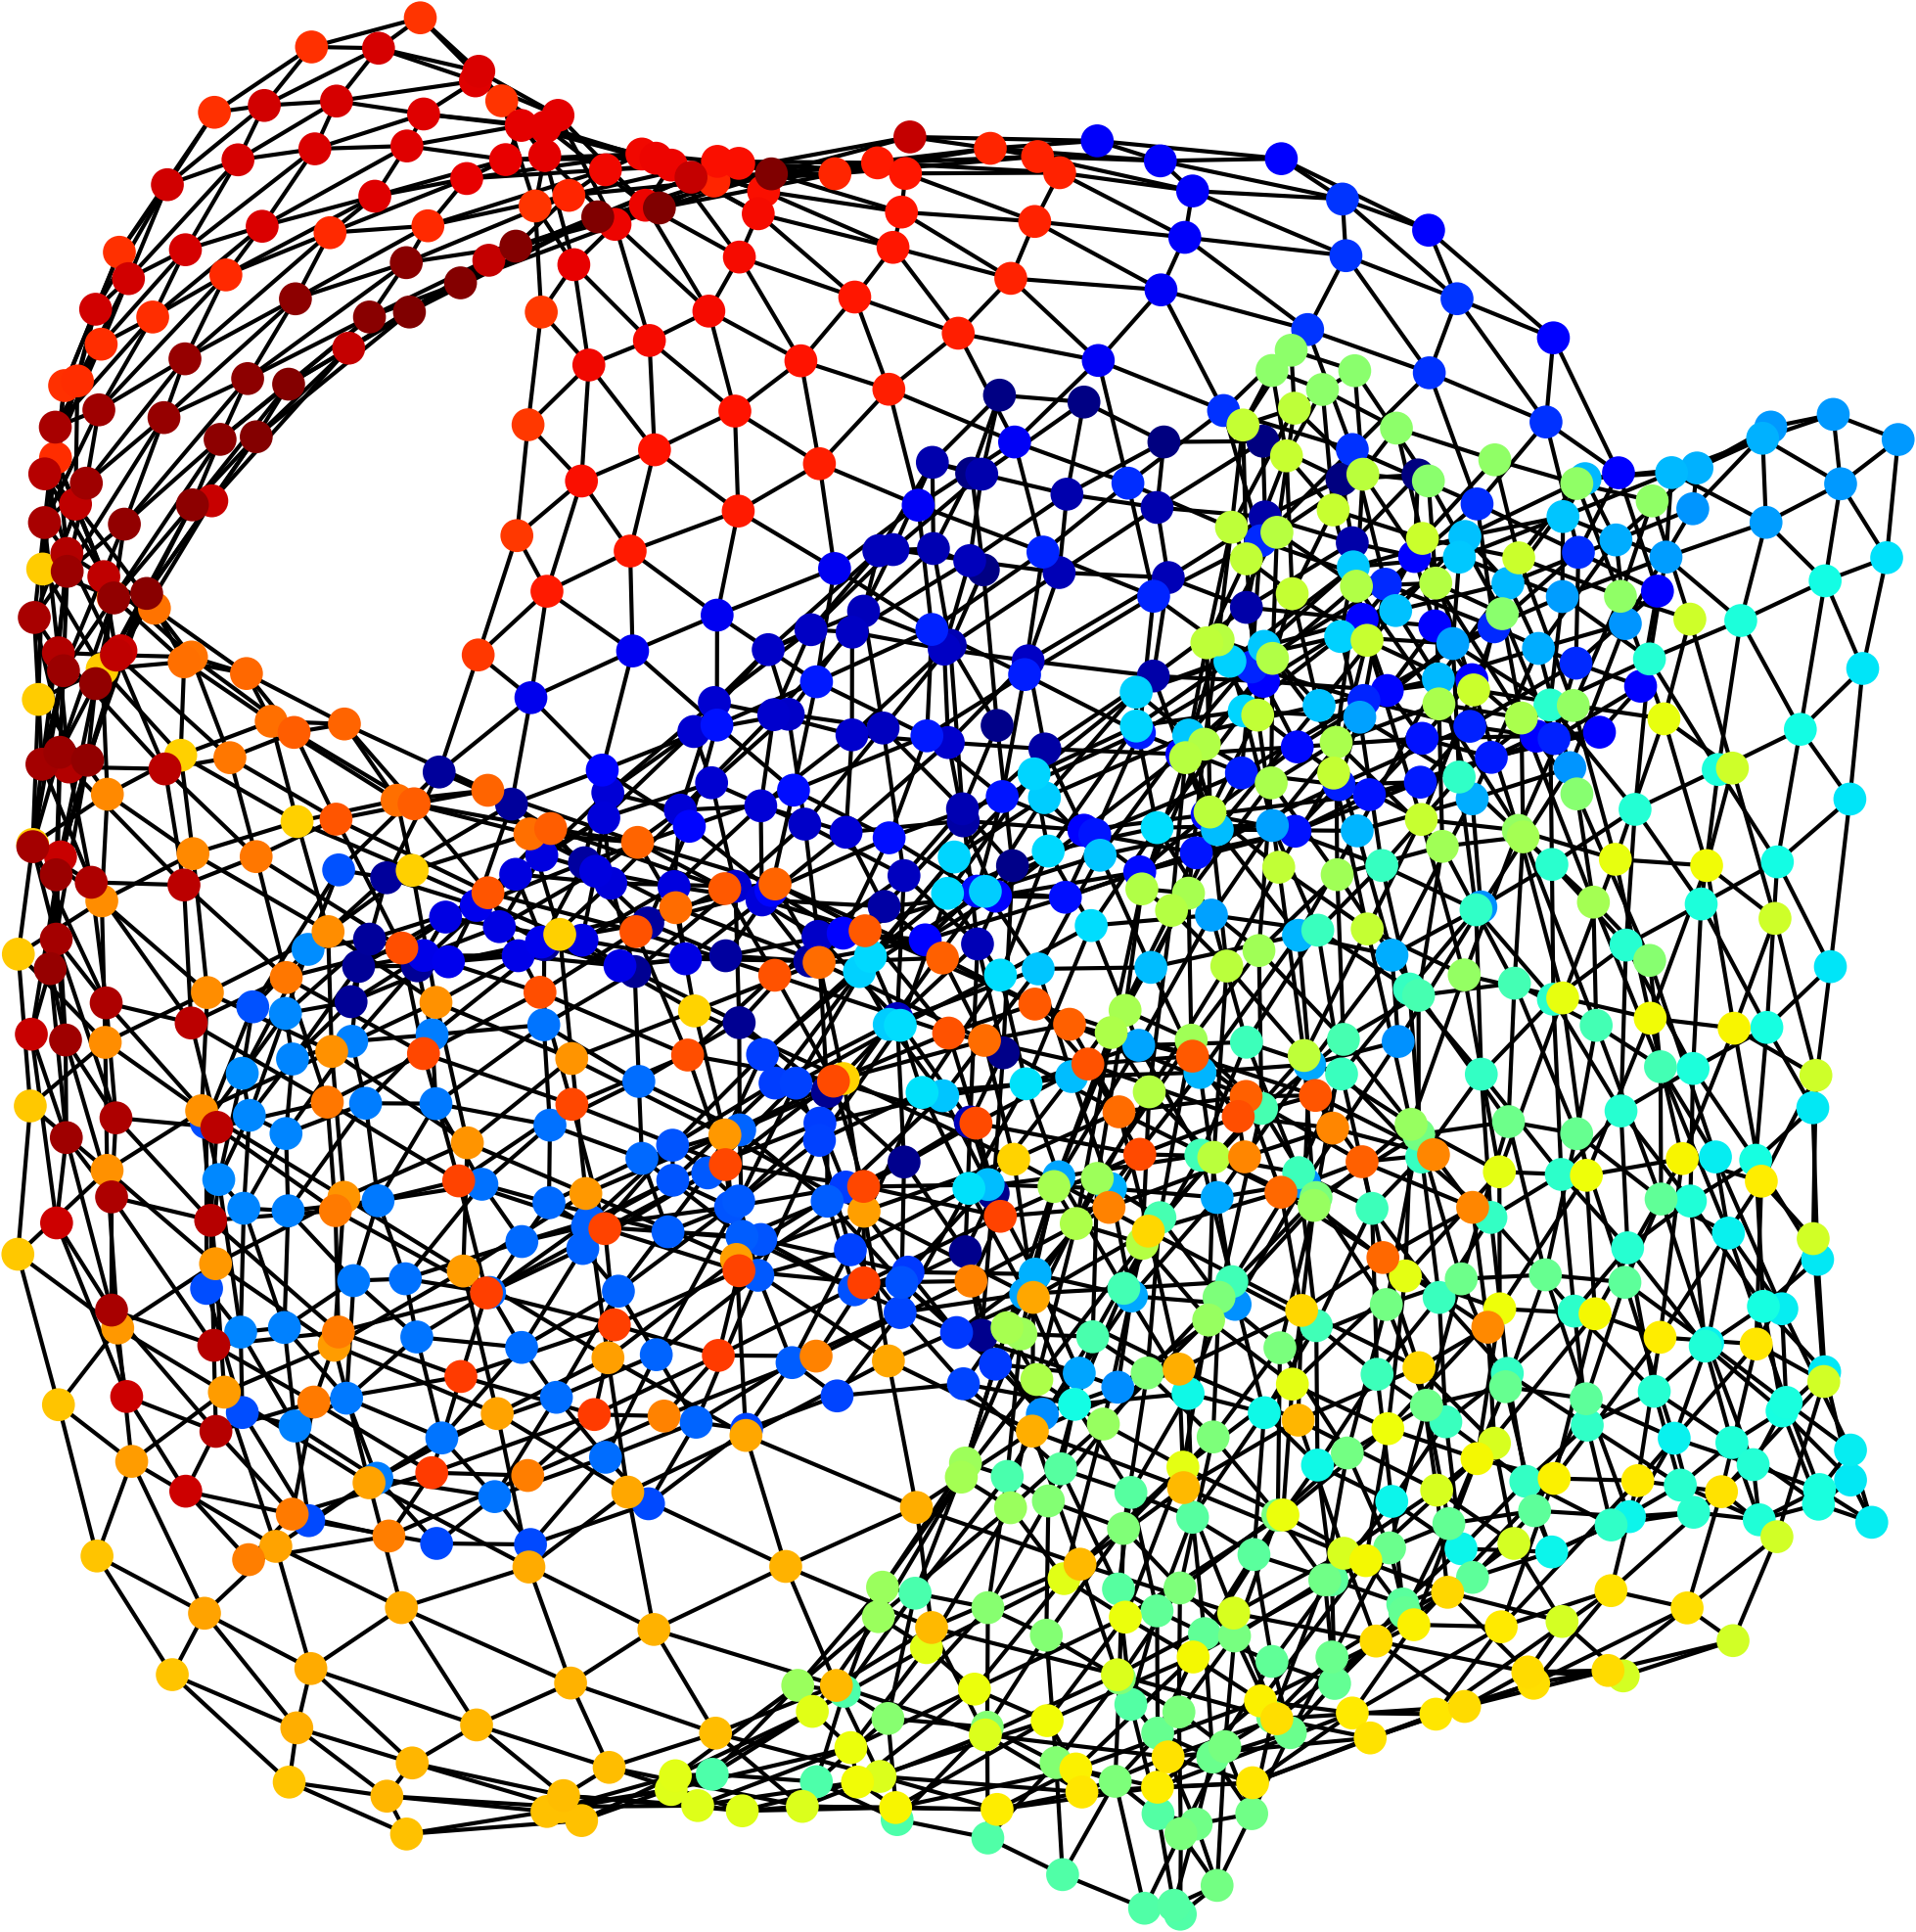
\includegraphics[scale=0.05]{jagmesh1_FR.png}
    \end{minipage} &
    \begin{minipage}{0.45\columnwidth}
      \centering
      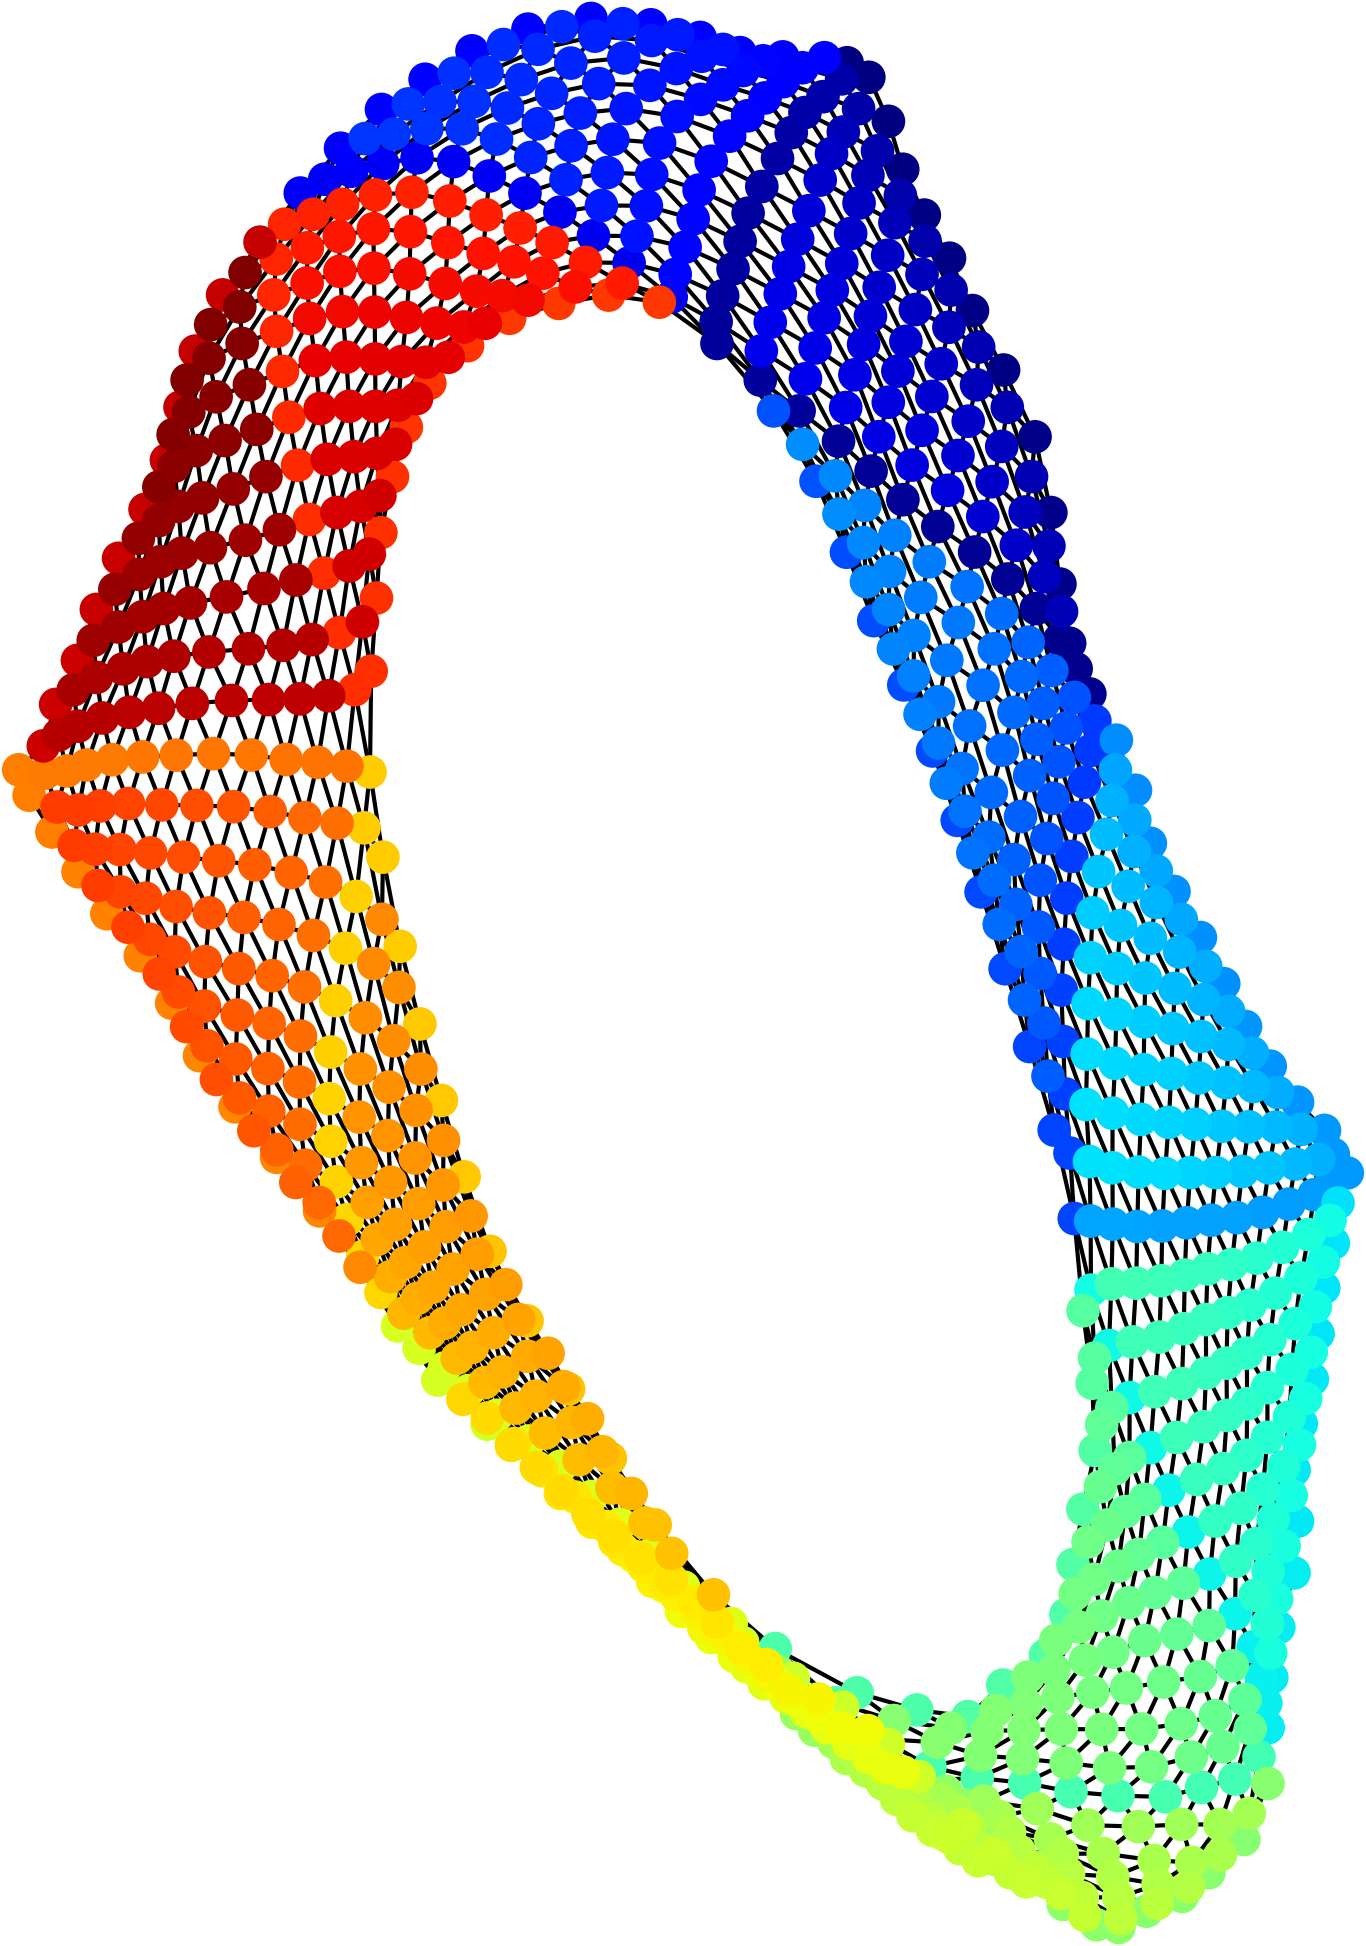
\includegraphics[scale=0.05]{jagmesh1_L_BFGS.png}
    \end{minipage}                          \\
    \large{\textbf{proposed}}                     & \large{\textbf{+ L-BFGS}} \\
    \begin{minipage}{0.45\columnwidth}
      \centering
      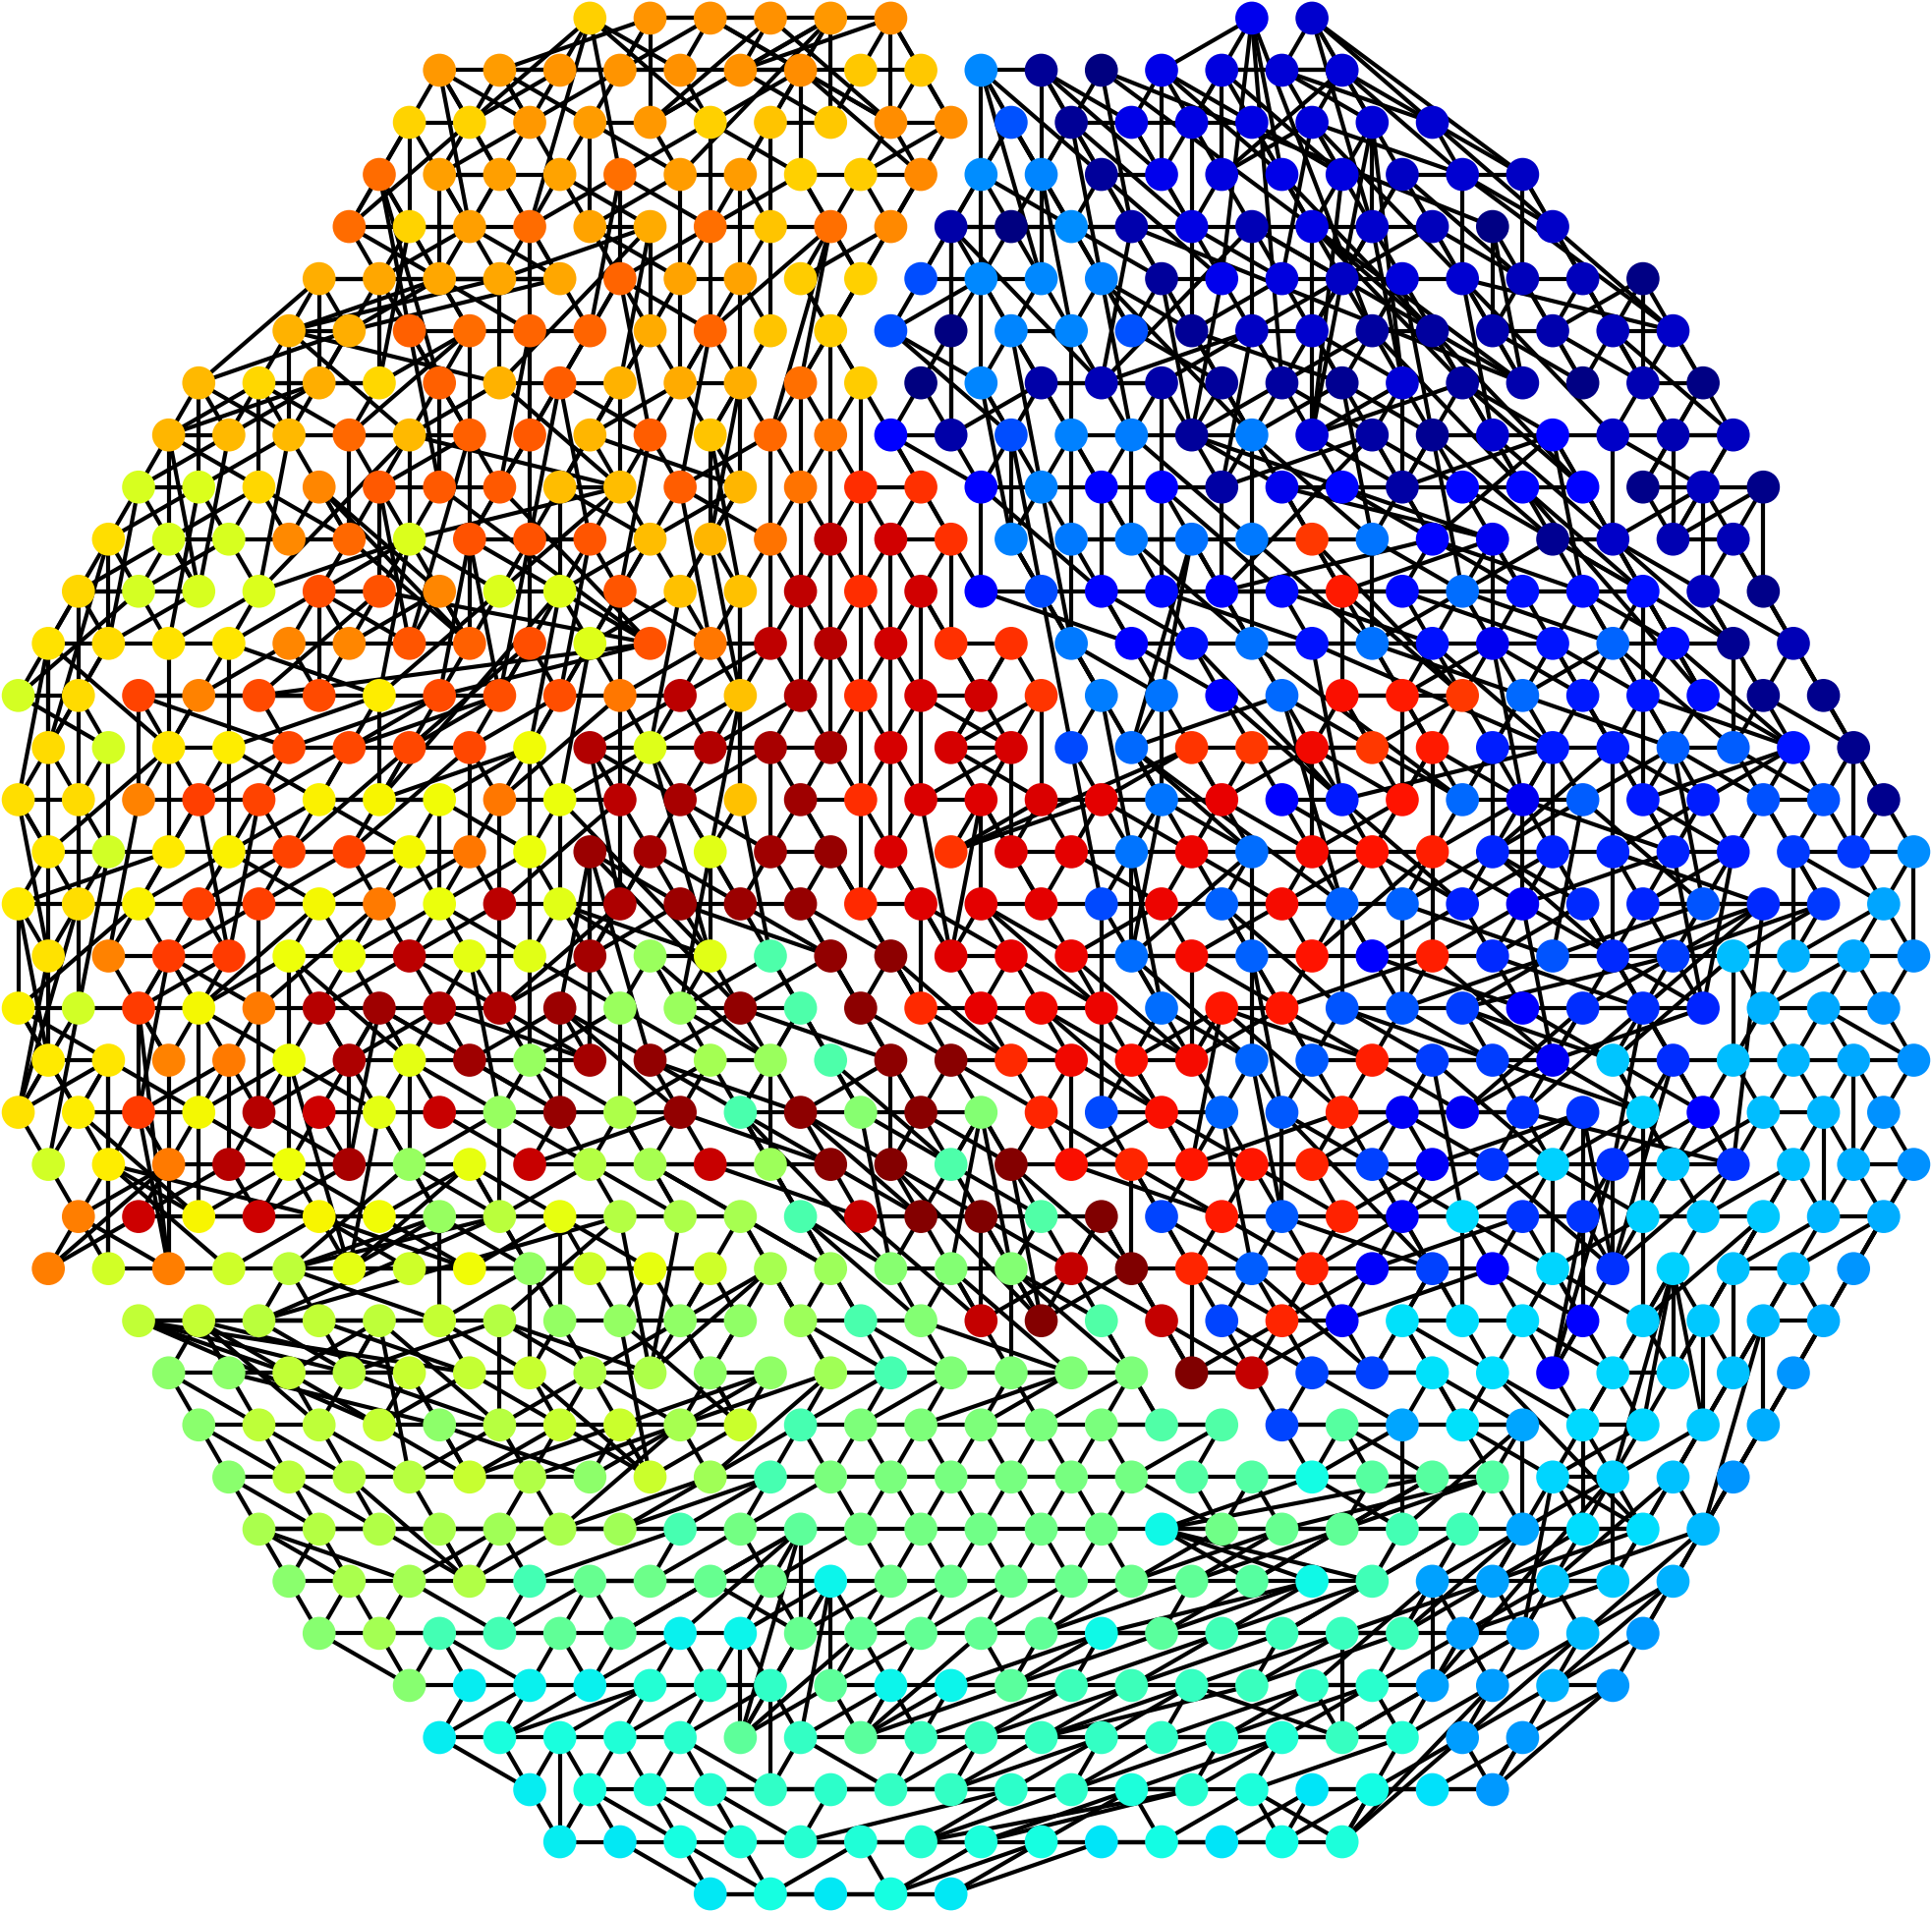
\includegraphics[scale=0.05]{jagmesh1_RS.png}
    \end{minipage}
                                                  &
    \begin{minipage}{0.45\columnwidth}
      \centering
      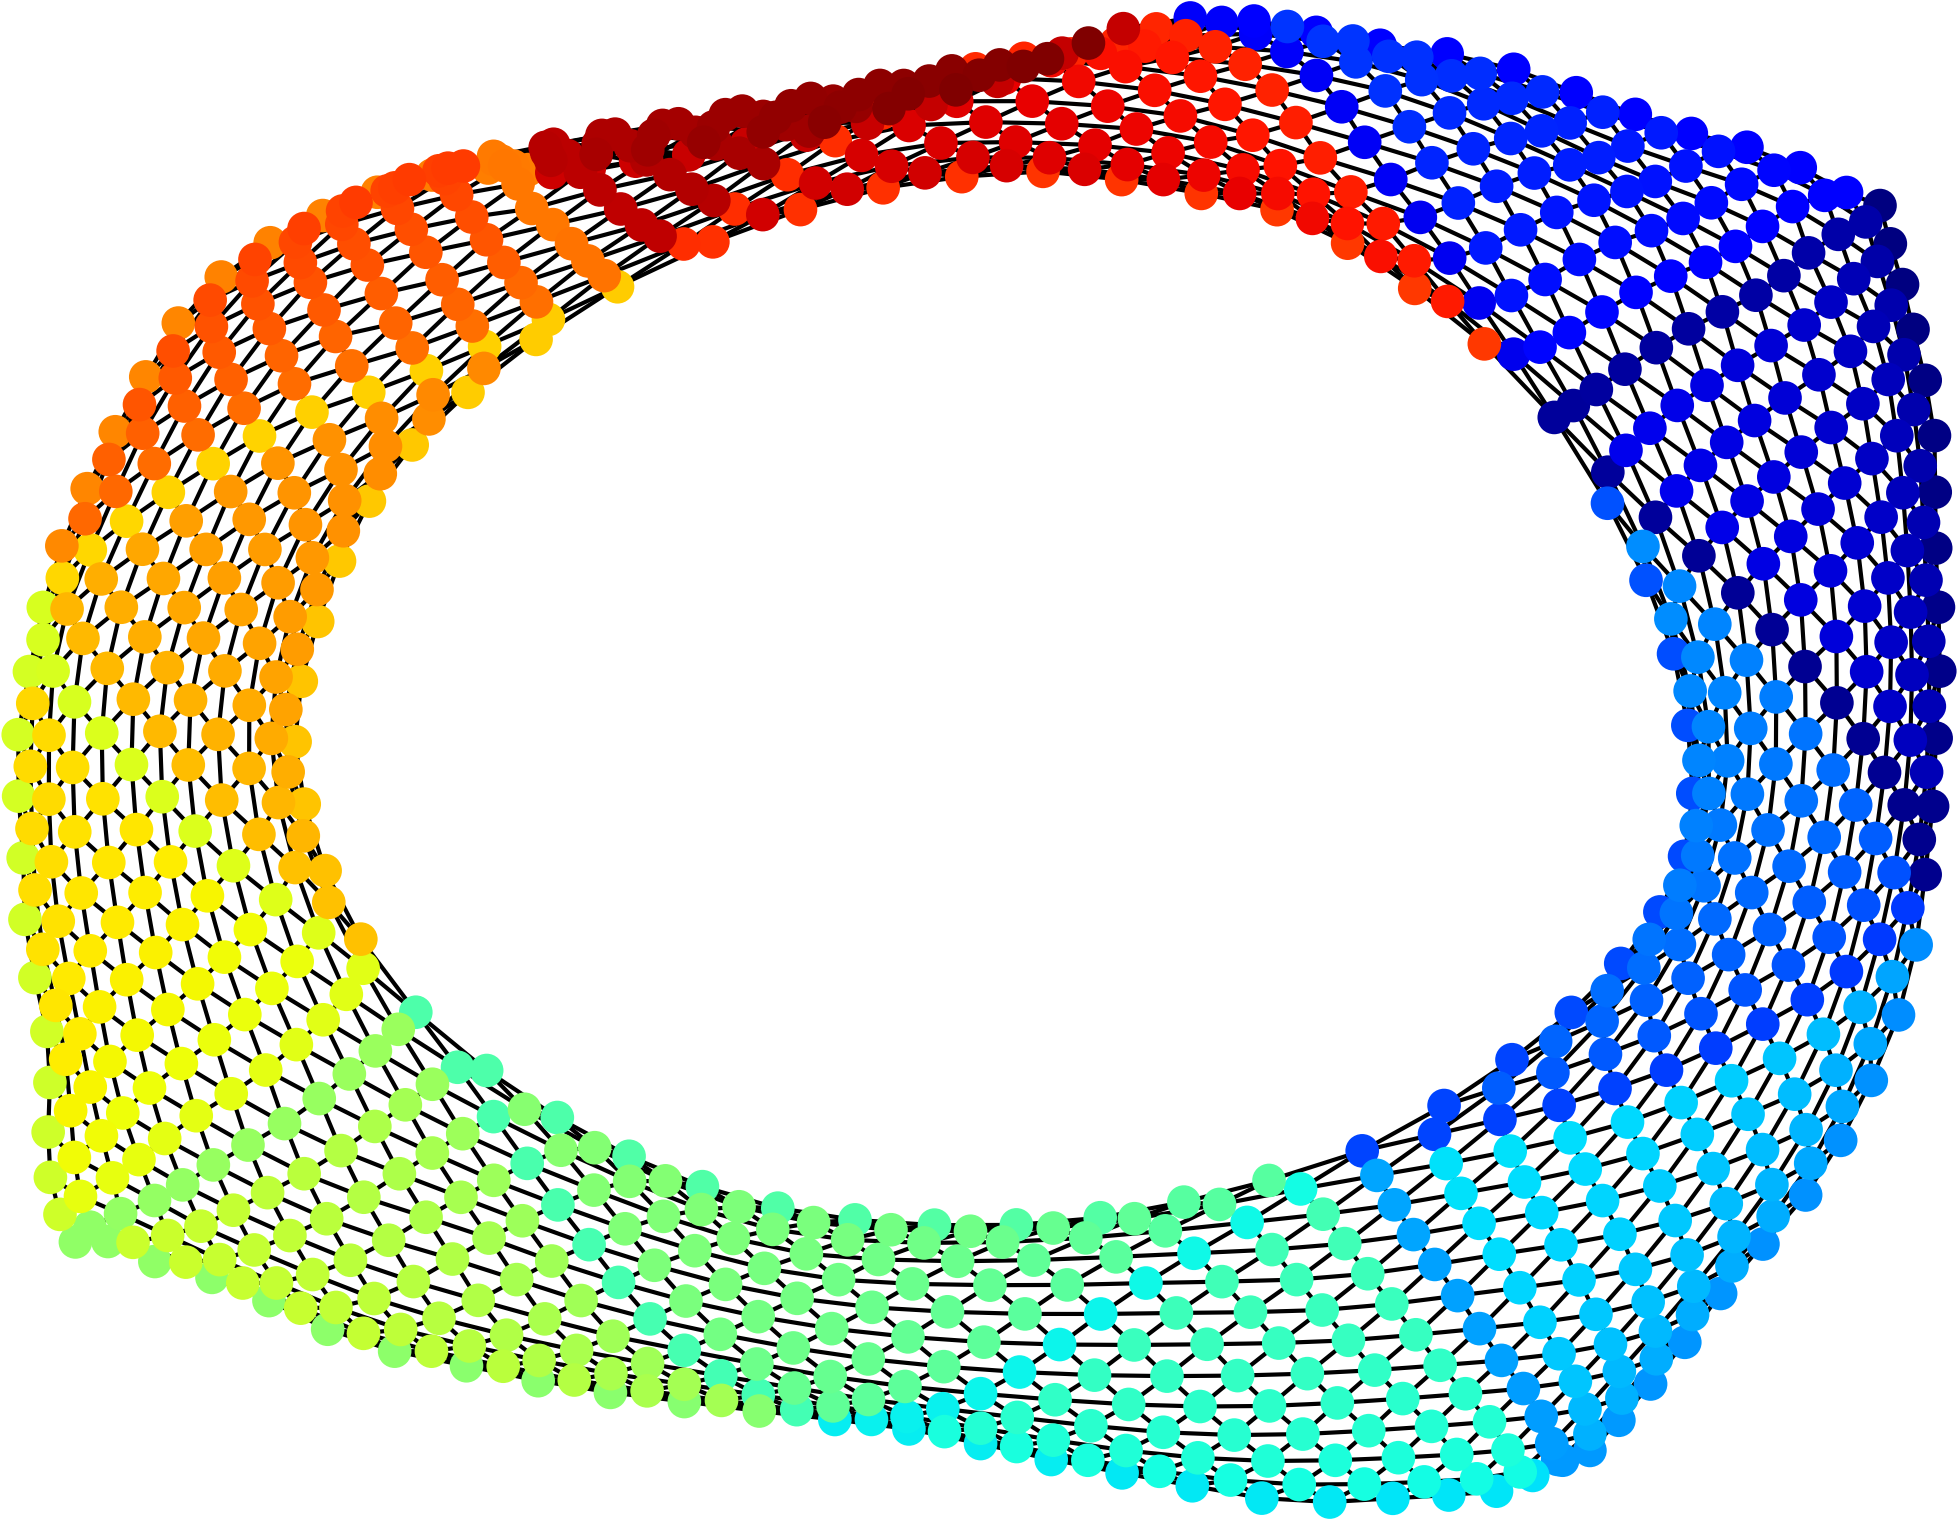
\includegraphics[scale=0.05]{jagmesh1_RS_L_BFGS.png}
    \end{minipage}
  \end{tabular}
  \begin{tikzpicture}[overlay, remember picture]
    \draw[->, thick] (-0.3,1.4) -- (+0.3,1.4);
  \end{tikzpicture}
  \caption{
    Comparison of the FR algorithm, L-BFGS, and the proposed method
    for the \texttt{jagmesh1} dataset.}
  \label{table:four_images}
\end{figure}

\section{Preliminary}\label{sec:preliminary}

\begin{figure}[t]
  \centering
  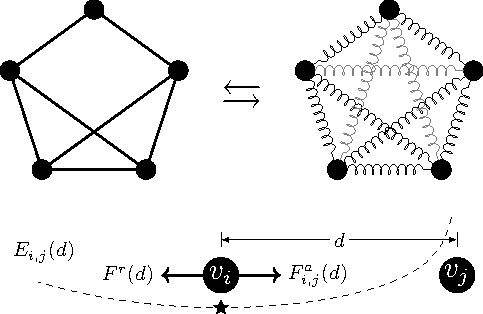
\includegraphics[height=5.5cm]{fr_layout.pdf}
  \caption{
    (Top) Fruchterman--Reingold layout. It models $\order{n^2}$ springs between all pairs of vertices.
    (Bottom) The equilibrium between attractive force $F_{i,j}^a(d)$ and repulsive force $F^r(d)$ is achieved at $d = k/\sqrt[3]{w_{i,j}}$, which equals $k$ when $w_{i,j} = 1$.
  }
  \label{fig:frLayout}
\end{figure}

In this section, we formulate the FR layout as a continuous optimization problem, and introduce the conventional approaches to this problem, namely the FR algorithm and the L-BFGS method.

\subsection{Fruchterman--Reingold layout}\label{ssec:frLayout}

Let $\bbR_{> 0} \defeq \qty{ x \in \bbR \mid x > 0 }, \quad \bbR_{\geq 0} \defeq \qty{ x \in \bbR \mid x \geq 0 }$, and let $W = (w_{i,j}) \in \bbR_{\geq 0}^{n \times n}$ be an adjacency matrix of a graph $G_W = (V, E)$, where $V = \qty{v_i \mid 1 \leq i \leq n}$ is a set of vertices and $E = \qty{(v_i, v_j) \mid w_{i,j} > 0}$ is a set of edges. We call $w_{i,j}$ as a weight of the edge $(v_i, v_j)$.

We will only consider undirected connected graphs with non-negative weights.
Although the FR algorithm in NetworkX, for example, can handle directed unconnected graphs with negative weights, this paper does not focus on such cases.
For directed graphs, slight modifications of algorithms or converting them to undirected graphs may be effective.
For unconnected graphs, algorithms can be applied to each connected component independently.
When negative weights are present, the optimization problem may become unbounded, but with non-negative weights and ensuring the graph's connectivity, the problem is always bounded and solvable.
In summary, the conditions for $W$ is formulated as follows:
\begin{equation}\label{eq:WCondition}
  W \in \bbR_{\geq 0}^{n \times n}, \quad W = W^\top, \quad \text{$G_W$ is connected}.
\end{equation}

Fruchterman and Reingold~\cite{fruchtermanGraphDrawingForcedirected1991} proposed a force-directed layout called the Fruchterman--Reingold (FR) layout, as known as a spring layout~\cite{osti_960616}.
Let $x_i \in \bbR^2$ be the position of the vertex $v_i \in V$, and $X = (x_1, \dots, x_n) \in \bbR^{2 \times n}$ be the configuration of the graph.
For a parameter $k$ and a distance $d_{i,j} \defeq \norm{x_i - x_j}_2$ between two vertices $v_i$ and $v_j$, the attraction force $F_{i,j}^a: \bbR_{> 0} \to \bbR$ and the repulsion force $F^r: \bbR_{> 0} \to \bbR$ is defined as
\begin{equation*}
  F_{i,j}^a(d) \defeq \frac{w_{i,j} d^2}{k}, \quad F^r(d) \defeq -\frac{k^2}{d}.
\end{equation*}
FR layout seeks the equilibrium of the forces between all pairs of vertices, as shown in Figure~\ref{fig:frLayout}.

We can also interrupt forces by its scalar potential~\cite{6183577}, in other words, energy $E_{i,j}: \bbR_{> 0} \to \bbR$, which is defined by
\begin{align}
  E_{i,j}(d) & \defeq \int_{0}^{d} F_{i,j}^a(r) \dd{r} + \int_{\infty}^{d} F^r(r) \dd{r} \notag \\
             & = \frac{w_{i,j} d^3}{3k} - k^2\log{d}. \label{eq:Eij}
\end{align}
As a remark, this energy function $E_{i,j}$ is convex as a function of $d$ and minimized when $d^* = k/\sqrt[3]{w_{i,j}}$, but it is not Lipschitz continuous and is not convex as a function of $x_i$. Refer to Figure~\ref{fig:energy3d}.

\begin{figure}[t]
  \centering
  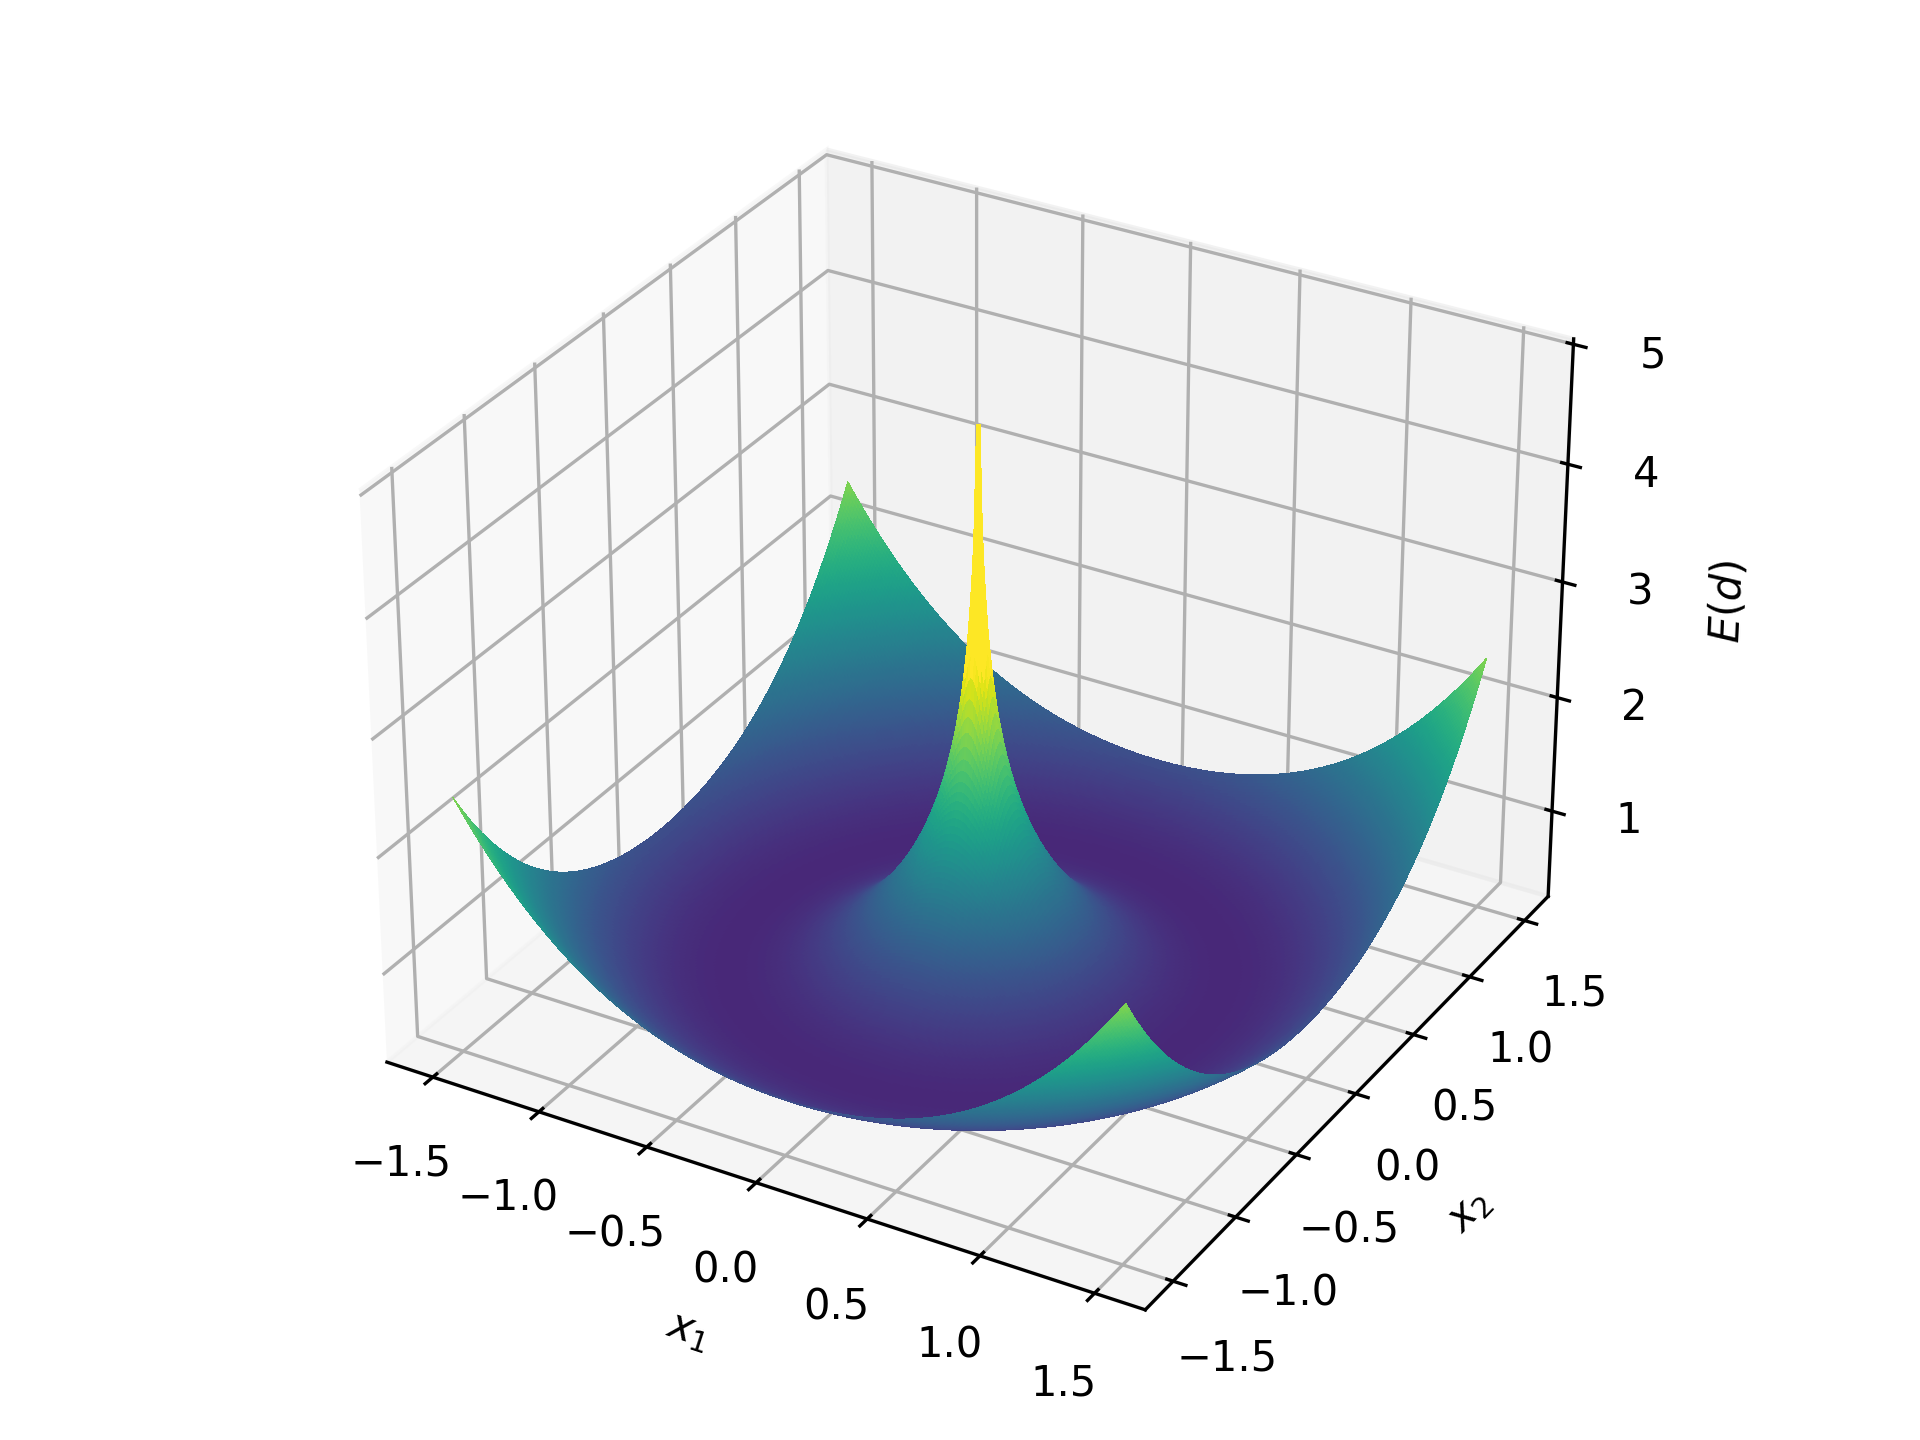
\includegraphics[height=5.5cm]{energy_3d.png}
  \caption{Energy function $E_{i,j}(d)$ for $x_j=(0,0)$, $w_{i,j} = 1$ and $k = 1$. Although $E_{i,j}$ is convex as a function of $d$, it is not convex as a function of $x_i$. As $x_i$ approaches $x_j$, the energy function diverges.}
  \label{fig:energy3d}
\end{figure}

Now, the optimization problem for FR layout can be formulated as the minimization of the energy function $f: \bbR^{2 \times n} \to \bbR$, as known as a stress of the graph:
\begin{mini}
  {X \in \bbR^{2 \times n}}
  {f(X) \defeq \sum_{i<j} E_{i,j}(d_{i,j}).}
  {\label{eq:fr}}
  {}
\end{mini}
This is because seeking an equilibrium of the forces is equivalent to minimizing the energy function $E_{i,j}$ for all pairs of vertices.
In the following, we will discuss the optimization of this problem.

\subsection{Fruchterman--Reingold algorithm}\label{ssec:frAlgorithm}

The Fruchterman--Reingold algorithm~\cite{fruchtermanGraphDrawingForcedirected1991}, the original force-directed algorithm for this layout, can be regarded as a most standard approach for solving the optimization problem~\eqref{eq:fr}.
As pointed out in~\cite{tunkelang1999numerical}, the FR algorithm can be regarded as a gradient descent method for the energy function $f$ with a cooling global temperature $t$.

Let denote $f_i(x): \bbR^2 \to \bbR$ as the energy function for the vertex $v_i$:
\begin{equation*}
  f_i(x_i) \defeq \sum_{j \neq i} E_{i,j}(d_{i,j}).
\end{equation*}
The gradient of $f_i$ is
\begin{equation}\label{eq:gradientFi}
  \nabla f_i(x_i) = \sum_{j \neq i} \qty(\frac{w_{i,j}d_{i,j}}{k} - \frac{k^2}{d_{i,j}^2}) (x_i-x_j),
\end{equation}
which is the sum of forces acting on the vertex $v_i$.

The pseudo code of the FR algorithm is shown in Algorithm~\ref{alg:fr}. It is based on the original implementation in~\cite{fruchtermanGraphDrawingForcedirected1991} and implementation in NetworkX~\cite{osti_960616} with some omitted details.

\begin{algorithm}[ht]
  \caption{Fruchterman--Reingold algorithm}
  \label{alg:fr}
  \KwIn{Graph $G_W = (V, E)$}
  \KwOut{Point configuration $X = (x_1, \dots, x_n)$}

  $\text{define parameters } k, t, dt, \text{iterations}$\;
  $x_i \gets \text{random position}$ for all $v_i \in V$\;
  \For{$j \gets 0$ \KwTo \textit{iterations}}{
    $\text{compute gradient } \nabla f_i(x_i)$ for all $v_i \in V$\;
    $x_i \gets x_i + t \frac{\nabla f_i(x_i)}{
        \norm{\nabla f_i(x_i)}_{2}}$ for all $v_i \in V$\;
    $t \gets t - dt$\;
    \If{\text{convergence condition}}{
      \textbf{break}\;
    }
  }
  \Return $X$\;
\end{algorithm}

In Algorithm~\ref{alg:fr}, the initial placement of points is determined randomly. Under proper input normalization, each point is uniformly distributed within a unit square in general.

The parameter $t$ denotes the temperature, which governs the step size of the gradient descent. As the temperature gradually decreases, the algorithm converges to a particular configuration, though this configuration is not necessarily the optimal solution.

\subsection{L-BFGS method}\label{ssec:lbfgs}

\begin{figure}[t]
  \centering
  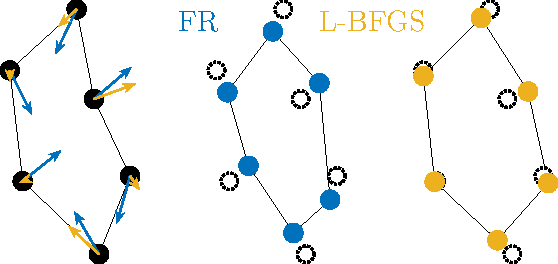
\includegraphics[width=0.804\columnwidth]{comparison_FRandLBFGS.pdf}
  \caption{
    For the graph on the left, which is in progress of L-BFGS, the FR algorithm and the L-BFGS method are executed for 1 iteration respectively.
    The L-BFGS achieves a lower $f(X)$, as it approximates the Hessian of $f$.
  }
  \label{fig:comparisonFRandLBFGS}
\end{figure}

Another approach to solve the optimization problem~\eqref{eq:fr} is to use the Limited-memory Broyden--Fletcher--Goldfarb--Shanno (L-BFGS) algorithm~\cite{6183577}.
The L-BFGS method is an optimization technique used for large-scale problems, which approximates the inverse Hessian matrix using only a few recent gradient vectors, making it more memory-efficient than the standard BFGS method (quasi-Newton method)~\cite{liuLimitedMemoryBFGS1989}.
This makes L-BFGS particularly suitable for high-dimensional optimization tasks. Since it is a more sophisticated method than the gradient descent method, the superior performance of the FR algorithm is reported in~\cite{6183577}. Also refer to Figure~\ref{fig:comparisonFRandLBFGS}.

There are many implementations of L-BFGS available, such as SciPy~\cite{2020SciPy-NMeth} and C++ L-BFGS~\cite{qiuYixuanLBFGSpp2024,okazakiChokkanLiblbfgs2024}, which we used in our experiments.

For the optimization problem~\eqref{eq:fr}, the L-BFGS method can be applied via flattening the configuration $X \in \bbR^{2 \times n}$ to a vector $\overline{X} \in \bbR^{2n}$.
However, it is worth noting that this method ignores the structure of $X$ and treats the problem just as a general optimization problem.
Thus, we can expect room for improvement by leveraging what we have ignored in this L-BFGS method.

\section{Research Question}\label{sec:RQ}

Now, we declare the research question of this paper: ``Can we accelerate the optimization process for the FR layout by leveraging the inherent structure of the problem?''.

In the previous section, we presented the FR algorithm and L-BFGS method. However, both methods face specific challenges during optimization, leading to inefficiencies and slow convergence, as detailed in Section~\ref{ssec:twist}.
Addressing these challenges forms a part of our research question, and we aim to introduce a new algorithm capable of overcoming these limitations. To achieve this, we will review key prior studies in Sections~\ref{ssec:sgd} and~\ref{ssec:introRSN}.

\subsection{twist in the optimization process}\label{ssec:twist}

\begin{figure}[t]
  \centering
  \begin{tabular}{ccc}
    \texttt{sfdp}                                             & \texttt{fdp} & \texttt{spring\_layout} \\
    
\includegraphics[width=0.27\columnwidth]{circle_sfdp.png} &
    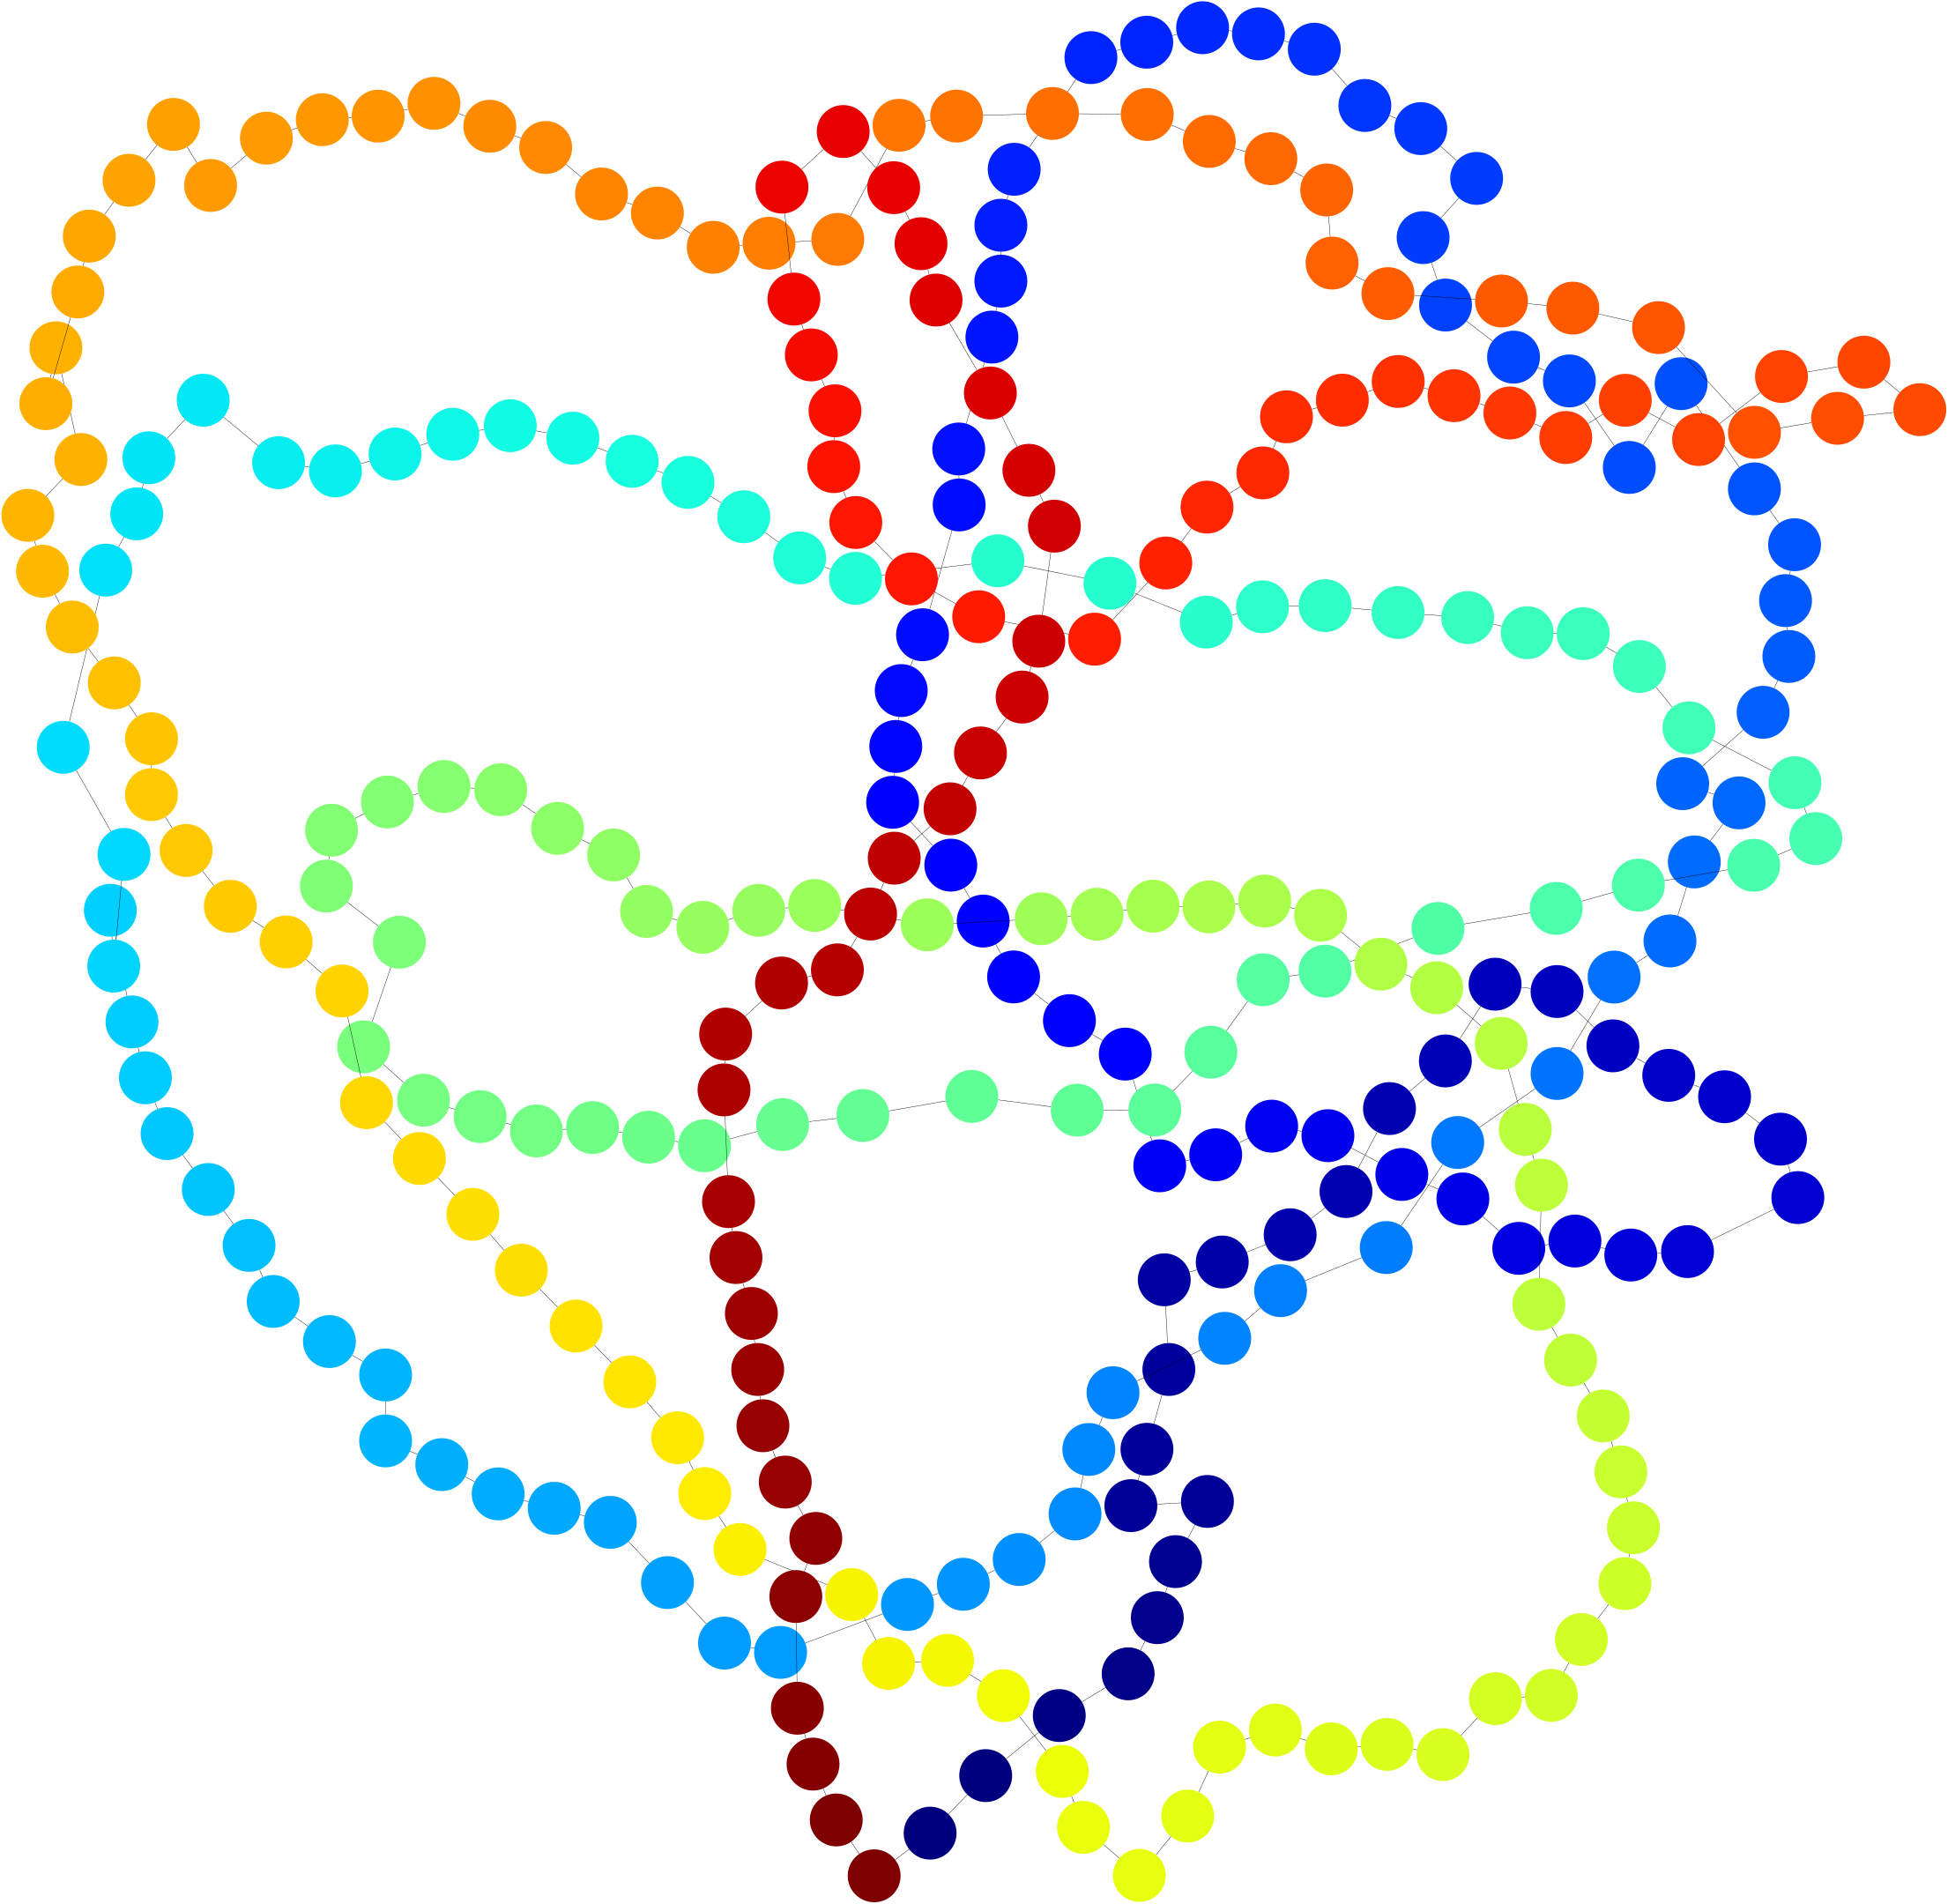
\includegraphics[width=0.27\columnwidth]{circle_fdp.png}  &
    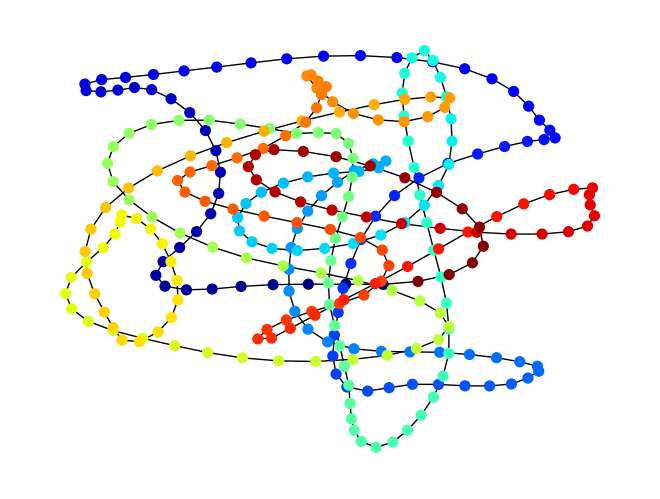
\includegraphics[width=0.27\columnwidth]{circle_fr.png}                                            \\
  \end{tabular}
  \caption{
    Comparison of \texttt{sfdp} in Graphviz, \texttt{fdp} in Graphviz, and \texttt{spring\_layout} in NetworkX for the circle graph with $\abs{V} = 300$.
    Every algorithm is run with the default parameters, but both \texttt{fdp} and \texttt{spring\_layout} fails to beautifully visualize the circle.
  }
  \label{fig:circle}
\end{figure}

First, we observe the challenges appeared in existing methods.
We identify that the most significant difficulty in optimizing the FR layout lies in resolving "twists".

The term "twist" does not refer to a mathematically rigorous concept; rather, it describes situations where unnecessary intersections of edges or tangled structures appear in visual representations.
Although the usage of the term "twist" is not common, it has been mentioned in works such as~\cite{cheongSnapshotVisualizationComplex2018}. Figure~\ref{fig:circle} illustrates a circle graph example of this situation.

The presence or absence of "twist" can impact optimization efficiency.
In the case shown in Figure~\ref{fig:circle}, even if vertices are disordered, optimization method proceeds relatively smoothly when no intersections between edges exist.
However, when "twist" exists, mutual interactions may diminish the gradient, causing the optimization to stagnate in typical continuous optimization processes, making it challenging to resolve the "twist".
Therefore, providing an initial placement of points that resolve "twist" as much as possible can significantly influence the efficiency of the optimization process.

\subsection{SGD for KK layout}\label{ssec:sgd}

Moreover, the effectiveness of Stochastic Gradient Descent (SGD) for Kama--Kawai (KK) layout is well-documented in~\cite{8419285}.
The KK layout is a energy based layout, which minimize the energy function $f^{\mathrm{KK}}$ defined as
\begin{equation*}
  f^{\mathrm{KK}}(X) = \sum_{i<j} f^{\mathrm{KK}}_{i,j}(d_{i,j}) = \sum_{i<j} \frac{k}{2}(d_{i,j}-l_{i,j})^2,
\end{equation*}
where $k$ is a constant, and $l_{i,j}$ is the optimal distance between them calculated from the shortest path distance in the graph.
The SGD method randomly selects pairs of vertices $(i,j)$ and adjusts their positions to minimize $f^{\mathrm{KK}}_{i,j}$ along the gradient direction, i.e. $x_i \gets x_i - \eta \nabla f^{\mathrm{KK}}_{i,j}(d_{i,j})$ and $x_j \gets x_j + \eta \nabla f^{\mathrm{KK}}_{i,j}(d_{i,j})$ with a learning rate $\eta$.

However, in contrast to the KK layout, the FR layout assigns the function $-k^2\log{d_{i,j}}$ to all $(i,j) \notin E$, making SGD relatively less effective for the FR layout.
Though, the superiority of SGD in the KK layout, which focuses on randomly selected edge, suggests that an optimization method focuses on randomly selected vertex may also be effective in the FR layout.
This observation motivates us to explore the application of Random Subspace Newton (RSN) to the FR layout as discussed in the next subsection.

\subsection{Introduction of Random Subspace Newton}\label{ssec:introRSN}

Now, we introduce the RSN method, which is not a proposed method itself, but a concept that heavily inspired our proposed algorithm.
The RSN method and its variant have been proposed in the context of optimization problems~\cite{NEURIPS2019_bc6dc48b,fujiRandomizedSubspaceRegularized2022,cartisRandomisedSubspaceMethods2022,higuchiFastConvergenceSecondOrder2024}.

First, we briefly explain the Newton's method.
For a convex function $f(x): \bbR^n \to \bbR$, the Newton's method updates $x$ by
\begin{equation*}
  x \gets x - \nabla^2 f(x)^{-1} \nabla f(x).
\end{equation*}
Since $f$ is convex, the Hessian matrix $\nabla^2 f(x) \in \bbR^{n \times n}$ is positive semi-definite, and the update direction is a descent direction. Plus, the updated $x$ is a optimal solution of the quadratic approximation of $f$ at $x$, which ensures the fast convergence of the Newton's method.
Newton's method requires to compute the inverse of Hessian matrix $\nabla^2 f(x)^{-1} \in \bbR^{n \times n}$ at each iteration, posing a high computational cost for large-scale problems.

In contrast, RSN focuses on a subspace of dimension $s$ randomly selected from the solution space by a projection matrix $P$ and utilizes the exact Hessian matrix of size $s \times s$ defined on this subspace: $P^\top \nabla^2 f(x) P$.
At each iteration, RSN updates the solution by
\begin{equation*}
  x \gets x - (P^\top \nabla^2 f(x) P)^{-1} P^\top \nabla f(x)
\end{equation*}
if $P^\top \nabla^2 f(x) P$ is non-singular.
Since $s \ll n$, the computational cost per iteration is significantly reduced when we can disregard the cost of selecting the subspace.

The RSN method resembles the stochastic coordinate descent method, which updates only a subset of the variables at each iteration using gradient information.
The difference is that RSN uses the Hessian matrix to determine the update direction, bringing the method closer to the Newton method.

Moreover, recent studies have explored its application not only to convex optimization problems but also to non-convex optimization problems~\cite{fujiRandomizedSubspaceRegularized2022}, using a regularization term to ensure the convergence of the method.

In particular, our problem~\eqref{eq:fr} exhibits a natural affinity with the RSN method, as it inherently defines a subspace of the solution space $X$ for the FR layout: $x_i \in \bbR^2$ for all $v_i \in V$.
Although its direct application to the FR layout is not effective as we depicted in Sec.~\ref{sec:problemRSN}, we exploit this idea in the proposed algorithm as discussed in the next section.

\begin{figure}[t]
  \centering
  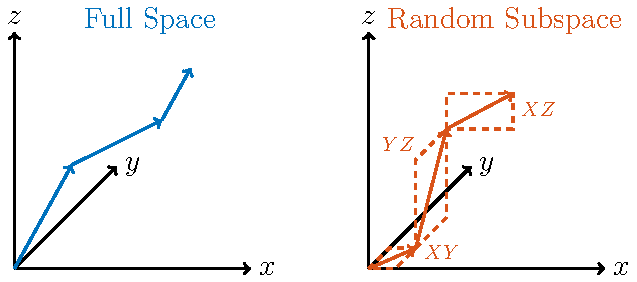
\includegraphics[width=\columnwidth]{randomSubspace.pdf}
  \caption{
    Visual explanation of Random Subspace Newton
    \orange{TODO}
  }
  \label{fig:randomSubspace}
\end{figure}

\section{Proposed Algorithm}\label{sec:algorithm}

Based on the research question above, we propose a new algorithm for the FR layout that utilizes the subspace method.
Our proposed method is described in three stages.
Firstly, in Section \ref{ssec:reduction}, we reformulate the optimization problem \eqref{eq:fr} into a simplified discrete optimization problem using a hexagonal lattice.
Secondly, in Section \ref{ssec:newtonDirection}, we present a method to solve the discrete optimization problem through continuous relaxation, using the Newton direction for vertices selected randomly, which is the core of our proposed algorithm.
Finally, in Section \ref{ssec:pseudoCode}, we show the complete framework of the proposed method, where the solution obtained from the previous step is used as the initial solution.

\subsection{reduction to the discrete optimization problem}\label{ssec:reduction}

First, we transform the optimization problem \eqref{eq:fr} into a constrained continuous optimization problem.
When $w_{i,j} = 0$, the energy function $E_{i,j}$ defined in \eqref{eq:Eij} becomes $-k^2\log{d_{i,j}}$.
Considering the sparsity of many practical graphs ($\abs{E} \ll \abs{V}^2$), simplifying as follow is a reasonable approach:
\begin{mini}
  {X \in \bbR^{2 \times n}}
  {f(X) = \sum_{(i,j)\in E} \frac{w_{i,j}d_{i,j}^3}{3k} - \sum_{i<j} k^2\log{d_{i,j}}.}
  {\label{eq:frApprox}}
  {}
\end{mini}
Further, by converting the second term into a constraint, the problem \eqref{eq:frApprox} can be approximated such that the objective function can be computed with a complexity dependent on $\abs{E}$ rather than $\abs{V}^2$:
\begin{mini}
  {X \in \bbR^{2 \times n}}
  {f^a(X) \defeq \sum_{(i,j)\in E} \frac{w_{i,j}d_{i,j}^3}{3k}}
  {\label{eq:frApprox2}}
  {}
  \addConstraint{d_{i,j}}{\geq \epsilon,\quad}{\forall (i,j)\,(i<j)}
\end{mini}
where $\epsilon$ is a suitably chosen positive constant. This conversion is reasonable because $-k^2\log{d_{i,j}}$ is a convex function such that decreases monotonically with respect to $d_{i,j}$. Thus, for sufficiently large $d_{i,j}$, the value of $-k^2\log{d_{i,j}}$ does not grow excessively, ensuring a validity of the approximation.

However, problem \eqref{eq:frApprox2} still involves $\order{\abs{V}^2}$ constraints, which negates the advantage of computing the objective function with $\order{\abs{E}}$ complexity.
To further simplify, we incorporate the concept of fixed initial configurations for the FR layout~\cite{ghassemitoosiSimulatedAnnealingPreProcessing2016}.
This study reports that a circular initial placement obtained by Simulated Annealing (SA) allows for \orange{a rapid derivation of an initial solution to the optimization problem.}
Similarly, by simplifying problem \eqref{eq:frApprox2}, we obtain the following discrete optimization problem:
\begin{mini}
  {\pi: V \to Q}
  {f^a(X) = \sum_{(i,j)\in E} \frac{w_{i,j}d_{i,j}^3}{3k}}
  {\label{eq:frApprox3}}
  {}
  \addConstraint{\norm{q_i - q_j}_2}{\geq \epsilon,\quad}{\forall q_i, q_j \in Q\,(q_i \neq q_j)}
  \addConstraint{x_i}{= \pi(v_i),\quad}{\forall v_i \in V}
  \addConstraint{\pi(v_i)}{\neq \pi(v_j),\quad}{\forall v_i, v_j \in V\,(v_i \neq v_j).}
\end{mini}
It means that, with a discrete set of points $Q$ such that the points are separated by at least $\epsilon$, we seek a best bijection $\pi$ from vertices $V$ to $Q$ that minimizes the objective function.
By fixing the possible point configuration in advance, the need to check the $\order{\abs{V}^2}$ constraints is eliminated, reducing the computational complexity to $\order{\abs{E}}$ and thus offering significant speedup.
This is exactly why we introduce a discrete optimization problem.

As an example of such a discrete point configuration $Q$, one could consider $n$ circles of radius $\epsilon$ packed in $\bbR^2$.
In this study, however, we adopt a hexagonal lattice.
The hexagonal lattice is known for its densest packing structure in space and offers computational simplicity.
Although not directly related to this study, prior research~\cite{s22145179} has also pointed out the connection between FR layouts and hexagonal lattices.
See Figure \ref{fig:pi} for reference.

\begin{figure}[t]
  \centering
  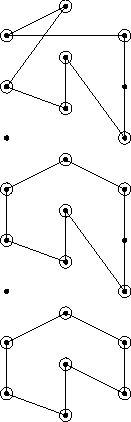
\includegraphics[width=\columnwidth]{pi.pdf}
  \caption{concept of $\pi$}
  \label{fig:pi}
\end{figure}

\subsection{the Newton direction for discrete optimization}\label{ssec:newtonDirection}

Next, using the Newton direction for a randomly selected vertex, we solve the discrete optimization problem through continuous relaxation. The computation of the Newton direction in this part is essentially identical to the RSN method described in Section~\ref{ssec:introRSN}.

Let the objective function $f^a_i(x_i)$ corresponding to a vertex $v_i$ be
\begin{equation*}
  f^a_i(x_i) \defeq \sum_{j \neq i} \frac{w_{i,j}\norm{x_i - x_j}_2^3}{3k}.
\end{equation*}
Using the Newton direction, we can solve the discrete optimization problem through continuous relaxation, i.e., by updating the position of a vertex $v_i$ as
\begin{equation*}
  x_i^\mathrm{new} \gets x_i - \nabla^2 f^a_i(x_i)^{-1} \nabla f^a_i(x_i),
\end{equation*}
Specifically, the position $x_i$ of the vertex $v_i$ is updated according to the Newton direction, and this new position is projected onto the nearest point on a hexagonal lattice, which is then taken as the new position of the vertex $x_i^\mathrm{new}$.
Additionally, by sequentially moving vertices from their original positions to the new ones, we can satisfy the constraints of the discrete optimization problem. The overall process is illustrated in Figure~\ref{fig:hex}.

Through this approach, a high-quality initial solution for the optimization problem~\eqref{eq:fr} can be obtained.

\begin{figure}[t]
  \centering
  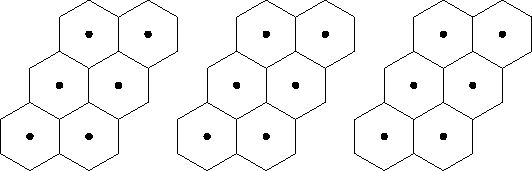
\includegraphics[width=\columnwidth]{hex.pdf}
  \caption{Visual explanation of the one iteration of the proposed algorithm. Step1. Compute the Newton direction for a randomly selected vertex. Step2. decide the path from the original position to the new position. Step3. move the vertex along the path.}
  \label{fig:hex}
\end{figure}

\subsection{pseudo code}\label{ssec:pseudoCode}

以上を基に、提案手法の全体像をアルゴリズム~\ref{alg:rsn}に示す。なお、このアルゴリズムの出力は、問題~\eqref{eq:fr}への解ではなく、離散最適化問題~\eqref{eq:frApprox3}の解であることに注意されたい。問題~\eqref{eq:fr}の解は、この出力結果に対し、さらにFR algorithmやL-BFGS methodを適用することで得られる。

\begin{algorithm}[ht]
  \caption{Proposed algorithm as as initial placement for the FR layout}
  \label{alg:rsn}
  \KwIn{Graph $G_W = (V, E)$, subspace dimension $s$}
  \KwOut{Point configuration $X = (x_1, \dots, x_n)$}

  define parameters $k, Q, \textit{iterations}$\;
  set $\pi$ as a bijection from $V$ to $Q$ randomly\;
  \For{$j \gets 0$ \KwTo \textit{iterations}}{
    $v_i \gets \text{randomly selected vertex from } V$\;
    $q_i \gets \pi(v_i)$\;
    $x_i^\mathrm{new} \gets x_i - \nabla^2 f_i(x_i)^{-1} \nabla f_i(x_i)$\;
    $q_i' \gets \text{nearest point of } x_i^\mathrm{new} \text{ in } Q$\;
    $\textit{path} \gets \text{path from } q_i \text{ to } q_i'$\;
    update $\pi$ by moving $q_i$ along the path\;
    \If{\text{convergence condition}}{
      \textbf{break}\;
    }
  }
  $x_i \gets q_i$ for all $v_i \in V$\;
  \Return $X$
\end{algorithm}

\section{Numerical Experiment} \label{sec:experiment}

In this section, we evaluate the proposed algorithm by various numerical experiments.
本実験は、Ref.~\cite{8419285}を参考に、次の二つの実験を行う:
\begin{enumerate}
  \item $\abs{V} = 100$のランダムグラフに対して、提案手法が有効であることを示す。
  \item $\abs{V} = 1000$のランダムグラフに対して、提案手法が有効であることを示す。
\end{enumerate}
We used dataset from \cite{davis2011university} and MatrixMarket \cite{boisvertMatrixMarketWeb1997}.

\subsection{Experimental Setup}\label{ssec:setup}
All numerical experiments in this paper were conducted using \Cpp17
compiled by GCC 9.4.0 and a cluster computer powered by Intel(R) Core(TM) i7-10510U CPU with 16 GB RAM.
All the codes are available at GitHub~\cite{Hamaguchi_stabilizer_extent_2024}.
The implementation about hexagonal grid is based on~\cite{patelHexagonalGrids2013}.

\url{https://reference.wolfram.com/language/tutorial/GraphDrawingIntroduction.html}

\subsection{網羅的な実験結果}\label{ssec:exprAll}
\subsection{詳細な実験結果}\label{ssec:exprDetail}

\section{Discussion} \label{sec:discussion}

In this sections, we discuss the results of the numerical experiments and the potential of the proposed algorithm.
Firstly, 我々は提案手法は、$\abs{V} \leq 1000$に対してのみならず、より大規模な問題に対しても適用可能であると考えている。その際に必要となる他のFR layoutの為の手法について、節~\ref{sec:combination}で述べる。
Secondly, 提案手法では元問題~\eqref{eq:fr}比べ、より複雑かつヒューリスティックな離散最適化問題~\eqref{eq:frApprox3}を経由したが、その理由について節~\ref{sec:whyDiscrete}で述べる。
Thirdly, 本研究のスコープであるグラフ描画を超えた、別のグラフ最適化問題に対する応用について、節~\ref{ssec:application}で述べる。
最後に、we conclude this paper in Section~\ref{sec:conclusion}.

\subsection{Combination with Other Techniques}\label{sec:combination}

\orange{todo: sfdpのアルゴリズムをきちんと述べる}

本論文では、$\abs{V} \leq 1000$なグラフに対して、提案手法が有効であることを示したが、より大規模な問題に対しても適用可能であると考えられる。
例えばGraphviz~\cite{ellsonGraphvizOpenSourceGraph2002}のScalable Force-Directed Placement (sfdp)では、$\abs{V}>1000$などのより大規模なグラフに対し、頂点の縮約を行う事で高速化を図っている。図~\ref{fig:circle}に示したsfdpの結果も、この手法の有用性を示している。
この頂点の縮約という操作は、本提案手法と衝突することなく、両者を組み合わせることが可能であると考えられる。具体的には、縮約後の$\abs{V}<1000$となるグラフに対して提案手法を適用することを繰り返せば、より大規模な問題に対しても適用可能であると考えられ、より高速かつより高品質な解を得ることができると考えられる。
このような取り組みは、今後の課題の一つとして挙げられる。

\subsection{何故離散最適化問題を経由するのか}\label{sec:whyDiscrete}

本研究では、離散最適化問題~\eqref{eq:frApprox3}を経由し、その問題に対する解をsubspace methodで求め、それを初期解として最適化問題~\eqref{eq:fr}を解く手法を提案した。
ここで、最も自然に湧き上がる疑問としては、何故元の問題~\eqref{eq:fr}に対してsubspace methodをそのまま適用せずに、離散最適化問題を経由するのかということが挙げられる。
これに対する答えは、Appendix~\ref{sec:}で詳述するが、ここでも簡単に述べる。

我々の考える答えは、本問題に対するsubspace methodは、大雑把に"twist"を減らすような目的に対して有効であるが、placement全体を最適化する目的には適していないから、ということである。
本研究で用いたsubspace methodでは、一つの頂点のみに着目して、
局所的に最善であることは、必ずしも大域的に最適であることを意味しない。故に、subspace methodをそのまま適用するだけでは、効率的に全体の最適解を求めることは難しい。

しかし、これは必ずしもsubspace methodの限界を意味するものではない、と我々は考えている。頂点毎に着目し最適化するというのは自然かつ妥当なアプローチ方法であり、subspace methodに更なる改良を加えることで、全体の最適解を効率的に求める可能性があると思われる。

\subsection{Application to Other Problems}\label{ssec:application}

グラフを基にした最適化問題は、グラフ描画問題以外にも多く存在する。
例えば、pair-wise separable functionとして分類され、最適化問題の一つとして扱われる問題がある。

今回提案した手法で核となるアイデアは、RSN methodの活用であり、頂点毎に最適化を行うことは有用であると実証された。

Originally, this kind of problems are solved by stochastic coordinate descent.
Random subspace algorithms might be applicable to these problems

例えば、グラフ描画の問題は、グラフ同型問題との関連性が深い。
(Continuous relaxation of) graph isomorphism problem
displaying symmetry is at least as difficult as graph isomorphism \cite{eades1984heuristic}
When we draw $G \defeq G_1 \cup G_2$, $G$ displays symmetry if $G_1 \cong G_2$.
Graph isomorphism problem with Frank-Wolfe algorithm \cite{klusContinuousOptimizationMethods2023}
\begin{mini*}
  {Q}{||QA-BQ||^2_F}{}{}
  \addConstraint{Q}{\in \left\{ Q \in \mathbb{R}^{n \times n} \relmiddle| Q^\top Q = I_n \right\}}
\end{mini*}
Many-to-Many graph isomorphism \cite{zaslavskiyManytoManyGraphMatching2010}
\begin{mini*}
  {P}{||G - PHP^\top ||^2_F}{}{}
  \addConstraint{P}{\in \left\{ P \in \{0, 1\}^{n \times n} \relmiddle| P1_n = 1_n, P^\top 1_n = 1_n \right\}}
\end{mini*}

\subsection{Conclusion} \label{sec:conclusion}

本研究では、FR layoutの最適化問題に対して、subspace methodを活用した新たな初期配置手法を提案した。また、その有効性を示すために、数値実験を行い、その結果、提案手法が$\abs{V} \leq 1000$なグラフに対して有効であることを示した。

提案手法が、FR layoutをはじめとするグラフ描画問題、
あるいはグラフにまつわる最適化問題に対し、
何かしらの示唆を与えることを期待し、
本論文を締めくくる。

\section{Acknowledgment}

The author would like to express our sincere gratitude to PL Poirion and Andi Han for their insightful discussions, which have greatly inspired and influenced this research.

\orange{networkXのdevelopment teamに感謝}

\orange{資金系のサポートについて}

\ifthenelse{\boolean{isMain}}{
  \bibliographystyle{IEEEtran}
  \bibliography{FruchtermanReingoldByRandomSubspace}
}{}

\appendices

\section{Optimal Scaling}\label{sec:scaling}

When we optimize a placement for FR-layout with an initial placement obtained, for instance through KK-layout, scaling the initial placement at first can often yield better results than directly using the unmodified initial placement.
In this section, we address the problem of finding the optimal scaling factor that minimizes the energy function for a given configuration.

\subsection{Optimal Scaling Algorithm}\label{ssec:scalingAlgorithm}

Formulating the optimization through scaling, the task reduces to selecting an appropriate scaling factor $x \in \bbR_{> 0}$ that minimizes the following energy function:

\begin{align*}
  \phi(x) \defeq {} & \qty(\sum_{i < j} \frac{w_{ij} (xd_{ij})^3}{3k}) - k^2 \sum_{i < j} \log(x d_{ij})                                     \\
  \begin{split}
    = {} & x^3 \qty(\sum_{i < j} \frac{w_{ij} d_{ij}^3}{3k}) - \log(x)(k^2 n(n-1)) \\
         & - k^2 \sum_{i < j} \log(d_{ij})
  \end{split} \\
  \phi'(x) = {}     & 3x^2 \qty(\sum_{i < j} \frac{w_{ij} d_{ij}^3}{3k}) - \frac{k^2 n(n-1)}{x}                                              \\
  \phi''(x) = {}    & 6x \qty(\sum_{i < j} \frac{w_{ij} d_{ij}^3}{3k}) + \frac{k^2 n(n-1)}{x^2}
\end{align*}

The function $\phi(x)$ is convex, and we can find the optimal scaling factor $x$ by using Newton's method.
\orange{This algorithm achieves sufficient convergence within a few iterations}, and when we pre-compute the coefficients of $\phi(x)$ with $w_{i,j} > 0$, the time complexity is just $\order{\abs{E}}$.

\section{Challenges of the Subspace method for the FR Algorithm}\label{sec:problemOfSubspace}

In this study, we proposed utilizing the subspace method as an initial placement. Then, a natural question can be arose: Can the subspace method alone achieve ``fast'' optimization throughout the entire process?
Specifically, we want to investigate whether the subspace method can optimize the positions of all vertices efficiently without the constraint of the hexagonal lattice.

To address this, we consider the following algorithm as a natural extension and application of the random subspace methods. Namely, we randomly select a vertex $v_i$, apply Newton's method to $f_i$ using Eq.~\ref{eq:gradientFi} and its Hessian:
\begin{gather*}
  \nabla^2 f_i(x_i) = \sum_{j \neq i} \left(\frac{w_{i,j}d_{i,j}}{k} - \frac{k^2}{d_{i,j}^2}\right) I_d + \\
  \sum_{j \neq i} \left(\frac{w_{i,j}}{k d_{i,j}} + \frac{2k^2}{d_{i,j}^4}\right) (x_i - x_j)(x_i - x_j)^\top.
\end{gather*}
Then, we update the position of vertex $v_i$, and repeat this process until convergence.
However, this approach fails to work effectively in practice.

We have reached a tentative conclusion that achieving ``fast'' optimization using the subspace algorithm alone is unlikely.
This section outlines some of the reasons behind this negative outcome.

It is important to note that these challenges do not necessarily imply fundamental limitations of the subspace method. On the contrary, improvements based on these identified issues could potentially enhance the effectiveness of the subspace method.

\subsection{Ignorance of other vertex movements}\label{ssec:ignorance}

L-BFGSを始めとする、問題全体のヘッシアンを考慮する手法は、ある頂点の位置を更新する際に、他の頂点の動きも考慮すると言える。ここでは、それがどのような意味を持つか論ずる。

\subsection{Inaccuracy of quadratic approximation}\label{ssec:inaccuracy}

まず、前提として、非凸であり、cubic regularized Newton methodをはじめとする正則化の追加が求められる。
しかし、そのような正則項

二次近似が著しく悪くなる場合がある。
しかし、subspaceに限定すると、特に問題が生じやすくなる。
その一例がFig.~\ref{fig:why_RSN_failed}で示すような状況である。

\begin{figure*}[t]
  \centering
  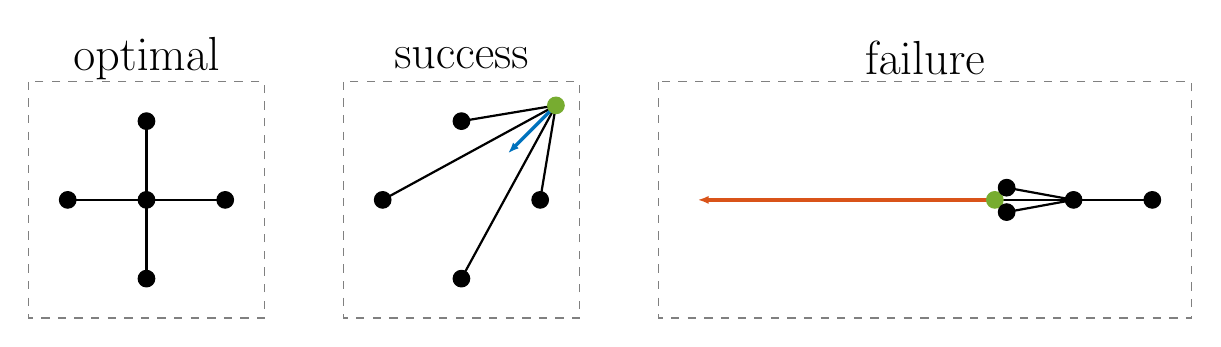
\begin{tikzpicture}
    \foreach \xA/\yA/\xB/\yB/\xC/\yC/\xD/\yD/\xE/\yE/\arrowX/\arrowY/\xShift/\xRect/\arrowV/\caZero/\caOne/\desc in {
        0/0/-1/0/0/1/0/-1/1/0/0/0/0/-1.5/a0/black/black/optimal,
        1.2/1.2/-1/0/0/1/0/-1/1/0/0.592271758813887/0.592271758813887/4/-1.5/a0/cC/black/success,
        0/0/-1/0/-0.85/0.155/-0.85/-0.155/1/0/-4.77422/0/11.77422/-5.27422/a1/black/cC/failure}{
        \begin{scope}[xshift=\xShift cm]
          \draw[dashed,color=gray,line width=0.5pt] (\xRect, 1.5) rectangle (1.5, -1.5);
          \node at ({(\xRect+1.5)/2}, 1.8) {\LARGE{\desc}};
          \coordinate (a0) at (\xA, \yA);
          \coordinate (a1) at (\xB, \yB);
          \coordinate (a2) at (\xC, \yC);
          \coordinate (a3) at (\xD, \yD);
          \coordinate (a4) at (\xE, \yE);
          \draw[thick] (a0) -- (a1);
          \draw[thick] (a0) -- (a2);
          \draw[thick] (a0) -- (a3);
          \draw[thick] (a0) -- (a4);

          \ifthenelse{\equal{\arrowX}{0} \AND \equal{\arrowY}{0}}{}{
          \ifthenelse{\equal{\desc}{success}}{
          \draw[-{Latex[length=4,width=3]},very thick,cA] (\arrowV) -- (\arrowX, \arrowY);
          }{
          \draw[-{Latex[length=4,width=3]},very thick,cD] (\arrowV) -- (\arrowX, \arrowY);
          }}

          \filldraw[draw=\caZero,fill=\caZero] (a0) circle (3pt);
          \filldraw[draw=\caOne,fill=\caOne]   (a1) circle (3pt);
          \filldraw[draw=black,fill=black] (a2) circle (3pt);
          \filldraw[draw=black,fill=black] (a3) circle (3pt);
          \filldraw[draw=black,fill=black] (a4) circle (3pt);
        \end{scope}
      }
  \end{tikzpicture}
  \caption{
    Visualization of the problem of the subspace method.
    Let a graph as shown in the left (optimal), where $k$ and all positive edge weights $w_{i,j}$ are set to 1.
    For the situation in the middle (success), the subspace method works effectively.
    However, in the situation depicted on the right (failure),
    where the points are set as $x_0=(0,0), x_1=(-1,0), x_2=(-0.85,0.155), x_3=(-0.85,-0.155), x_4=(1,0)$,
    the Hessian for the subspace of $x_1$ is approximately
    $
      \begin{pmatrix} 1.841 & 0 \\ 0 & 1.159 \end{pmatrix}
    $.
    This Hessian, while positive definite and not ill-conditioned, leads to a Newton direction that clearly deviates significantly from the global optimal solution.
  }
  \label{fig:why_RSN_failed}
\end{figure*}

However, unfortunately, the RSN method is not necessarily effective for the FR layout.
As shown in Figure \ref{fig:why_RSN_failed}, although the energy function \( f_i \) with respect to the position \( x_i \) of each vertex is convex in the FR layout, the overall energy function \( f \) with respect to \( x_i \) is not convex.

これに対する解決策として、line searchの実施などである。しかし、そもそものNewton directionが最適解から大きく外れるという問題は、必ずしも解決できない可能性があることには注意されたい。

\section{Another approach based on the Proposed Method}\label{sec:anotherApproach}

本論文では六方格子に基づいたSubspace Methodを提案したが、基本的に同一のアイデアに基づいた他のアプローチも考えられる。

\subsection{Non-randomized approach}\label{ssec:nonRandom}
一つは、各頂点毎に最適化する際に、ランダムに頂点を選んで最適化していくのではなく、$\abs{V}$点全てを同時に最適化する方法である。

こうすることによって、六方格子という制約をよりラフに扱うことが出来る。

六方格子への射影は、MinCostFlowなどで$\order{\abs{V}^3}$で厳密解が出せる。
ソートによる擬似的な射影で、$\order{\abs{V} \log \abs{V}}$で近似解が出せる。

\subsection{Non-Newton approach}\label{ssec:nonNewton}

もう一つは、Newton法を使わずに、勾配法を使う方法である。

以上のいずれも、基本的に性能は落ちると考えているが、実装が簡略化するなどの利点や、イテレーション毎の計算コストが多少減るという利点があり、検討の余地が残されている。

\begin{IEEEbiography}[{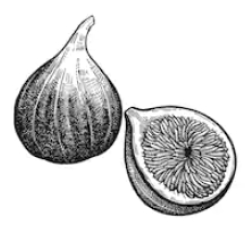
\includegraphics[width=1in,height=1.25in,clip,keepaspectratio]{fig1}}]{Hiroki Hamaguchi}
  Graduate School of Information Science and Technology, The University of Tokyo, Tokyo, Japan.
\end{IEEEbiography}
\begin{IEEEbiography}[{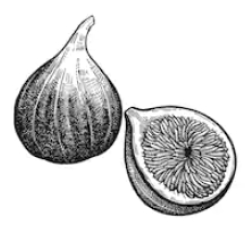
\includegraphics[width=1in,height=1.25in,clip,keepaspectratio]{fig1}}]{Naoki Marumo}
  Graduate School of Information Science and Technology, The University of Tokyo, Tokyo, Japan.
\end{IEEEbiography}
\begin{IEEEbiography}[{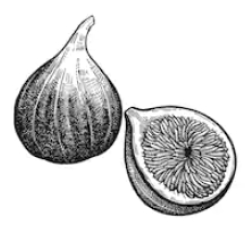
\includegraphics[width=1in,height=1.25in,clip,keepaspectratio]{fig1}}]{Akiko Takeda}
  Graduate School of Information Science and Technology, The University of Tokyo, Tokyo, Japan.
  Center for Advanced Intelligence Project, RIKEN, Tokyo, Japan.
\end{IEEEbiography}

\end{document}